\documentclass[10pt,b5paper,twoside,openright]{book}
%Template for project and MSc project reports created by MSc Morten Fyhn Amundsen
\usepackage{graphicx}
\graphicspath{ {report/figures} }

\usepackage{config}


\begin{document}


% \frontmatter
% \pagestyle{plain}
% \begingroup
% \let\cleardoublepage\clearpage
% %Problem description - describing the project tasks, supervisor and co-supervisor - is the first page of the report. For MSc theses this is generated by the DAIM system. For project reports, you generate this page yourself.
% %!TEX root = ../Thesis.tex
\chapter*{\englishabstractname}
\addcontentsline{toc}{chapter}{\englishabstractname}

Much research can be found on condition monitoring for many industries. There are, however, very little research on the use of condition monitoring in hydroelectric power plants. Most of the existing research involves methods that require both normal and abnormal data, and need data for all failure modes that one want to monitor. A literature study investigates this field, and it is found that support vector machines and neural networks have been successfully used for condition monitoring of known failure modes. 

Anomaly detection is presented as it enables the detection of anomalies in the process data, with only normal process data available. Three different methods for anomaly detection are presented, support vector machines, kernel density estimation and long short term neural networks. In addition, different techniques for feature and dimensionality reduction are presented. A data set containing data from 27 power plants is analyzed, and a reported incident with operational problems for the needles of a Pelton turbine is extracted for analysis. Data from two different plants and three different turbines are included in the analysis to investigate cross plant performance. An artificial error replicating the operational problems for the reported incident is created to verify how early the anomaly detection techniques can detect system degradation. In addition, two Pelton turbine start failures are included in the analysis to verify that the methods correctly detect abnormal system data. 

All three methods are shown able to detect the operational problems for the Pelton needles. However, the one class support vector machine is shown to very dependent on the choice of hyperparameters with regards to the training data. Kernel density estimation and long short term recurrent neural network show better performance and are more robust with regards to parameterization and training data. It is also shown that they can detect the early signs of the system degradation seen leading up to the reported incident with the Pelton needles. 

\clearpage

% %!TEX root = ../Thesis.tex
\chapter*{\norwegianabstractname}
\addcontentsline{toc}{chapter}{\norwegianabstractname}
%
Sammendraget skal gi en kort oppsummering av innholdet i rapporten.
%
\clearpage

% \tableofcontents \clearpage
%List of Acronyms, and List of symbols can be useful to include if you have many.
\endgroup

\mainmatter
\pagestyle{headings}
%!TEX root = ../Thesis.tex
\chapter{Introduction}\label{cha:introduction}
%
% This introductory chapter will briefly provide context for the material/results presented in this report and give motivation and a description of the problem to be solved. A literature review summarizes existing relevant knowledge and establishes the foundation of the later control system. The scope of the work is then defined by a list of assumptions. Finally, the contributions of the thesis are defined and elaborated.

This is a master thesis written in cooperation between NTNU and Hymatek Controls. Hymatek Controls is located in Oslo and delivers equipment and control systems to hydroelectric power plants worldwide. Hymatek is increasing its focus on condition monitoring and anomaly detection, and has acquired a large dataset containing data from a five year period for $27$ hydroelectric power-plants. The goal of this thesis is to find possible use cases for condition monitoring in the provided dataset, research possible techniques and implement some of them in the found use case. Since this is a new research area for Hymatek, this thesis will cover a wide range of aspects. 

This chapter provides an introduction to the work done, describing the motivation and problem description for the thesis. In addition, a literature review looking into state of the art techniques used for condition monitoring. Finally, the outline of the report is presented. 


\section{Motivation}\label{sec:motivation}

% % What is the motivation for considering the problems/question that you approach in your work? Why is this an interesting problem? The motivation should instead describe why it is interesting from a societal point of view, and/or from a scientific point of view.

The need for renewable and stable energy sources is great in Norway, Europe and worldwide. According to \cite{Statkraft2009} $99\%$ of the Norwegian power production comes from hydroelectric power plants. Almost $50\%$ of Europe's hydroelectric capacity is located in Norway. Hydroelectric power is seen as one of the most stable and cleanest energy sources one can find \cite{Statkraft2009}. Hydroelectric power plants have a high investment cost, but according to \cite{Selak2014} operation and maintenance costs are as low as 2\% of the cost of the initial investment, this makes it one of the cheapest energy sources one can find. As many European countries are transitioning into renewable energy sources, the need for stable and controllable power sources grows. Both wind and solar power production are dependent on weather conditions, and their production capacity can change quickly and unexpectedly. Norway has been called Europe's renewable battery due to its hydroelectric capacity, and the power delivery capacity is growing. By 2021 Norway and Great Britain will be connected through a new underwater power cable. This is an example that shows that Norway is becoming a part of a more complex energy market. As the exporting capacity grows, green energy from Norway can be supplied to reduce the consumption of fossil energy from for example coal from the European continent. This means that increased productivity and efficiency in hydroelectric power plants effectively can help make the green shift in the European power production happen. 

One way to increase a plant's productivity, is to ensure that it is operable at all times. This is however not possible since one has to perform maintenance on all parts of a plant. Planned maintenance is however not the only reason for a power plant stopping down. Components can breakdown outside of their service interval, leading to unplanned downtime. This is of course not only a case for hydroelectric power plants but for more or less any industry or factory. Unplanned downtime is expensive for the energy company that operates the plant, and depending on the time of year and the duration of the breakdown, the cost can have a large impact on their operation. Finding a way to avoid these breakdowns, and replacing unplanned maintenance with planned maintenance, is something all energy companies are interested in. A hydroelectric power plant contains several large components such as turbines, generators, transformers, hydraulic systems, valves, pipes etc. In addition, you have all the equipment needed to operate the plant. Keeping spare parts for all components would require an enormous storage, in addition to tying large assets due to the cost of all components. In addition, many components don't need to be replaced often, hence the spare can be left in storage for many years, and may even never be replaced. Clearly, this is not an optimal solution. 

Another approach is to try to eradicate unexpected breakdowns. This means that one needs to have a way to detect that a component is decaying so that one can plan an overhaul or replacement before it breaks down. This also solves another factor to consider when it comes to breakdowns of components, the domino effect. Depending on the situation and the component, if one component breaks down, it might end up taking several other with it. If a bearing on a turbine shaft breaks down, one risks that the damage will spread to the bearing on the other side of the shaft, and even to the turbine and generator. A continuous analysis of the condition of the bearing could help avoid this issue. This is known as condition monitoring. In its most complete form, condition monitoring gives an insight into the condition of the monitored components, giving an estimate to the remaining lifetime of the component. Introducing condition monitoring could help reduce the number of breakdowns, as components can be replaced before breaking.

There are many good reasons for pursuing the topic of this thesis, on a personal level it is motivating to work with real-world data, to learn the difference between theoretical and practical engineering. Looking for solutions that will improve the operation of a hydroelectric power plant, which can give even more clean energy is also motivating. Additionally, the fact that possible solutions found for the specific cases looked into most likely can be adapted to other industries is also very motivating. 

% An attempt of classifying the wear of the guide vanes on a Francis turbine was performed in my project thesis.  


% This triggered my interest in the possibilities of information found in data. 
% Looking into different possible techniques for condition monitoring that can be utilized on a real-world dataset will give
% As the world becomes more and more digitized, one can either keep up or be left behind. Condition monitoring is seen as an important part of the future portfolio of Hymatek Controls and a necessary addition to continuing their growth into the future. 

% \section{Contributions}
    


\section{Problem definition}

% Korleis oppsto problemstillinga? dreiv å såg gjennom feiloggen etter interesssante feil. Såg då at det var problemer med nålstryinga for hjartdøla. Starta så å undersøke dataen, og fant etterkvart ut at det er 2 anlegg til som har nålstyring. Dei hadde derimot ikkje raportet feil med nålene, noko som gav meg grunn til å tenke at dei har normal oppførsel. Då kunne eg og starte å samanlikne data mellom kraftverka for å sjå kva som er unormal og normal oppførsel.

No exact problem definition was provided by Hymatek, they provided a dataset containing process-data from $27$ hydroelectric power plants for the period $2013-2017$, and gave no restriction on which plants and cases that could be investigated. A historical incident log was also provided for all plants, with varying level of detail. Based on this, the problem definition was split into three main parts. As this is a thesis built upon an unknown dataset with unknown quality, an important factor is to recognize what the data can be utilized for, and what improvements that could/ need to be done to make the data analysis more extensive. Ideally, the result of the thesis will be a system for condition monitoring for a real-world case found in the dataset. However, since Hymatek is still in the start-up phase of its condition monitoring research, all experiences from this thesis are valuable. Therefore the most important part of the thesis is to understand why or why not one is able to create a condition monitoring system for the given case. Then this thesis can be used as a basis for further condition monitoring case analysis. The three parts are as follows: 

\begin{itemize}
    \item Finding techniques and methods for condition monitoring and anomaly detection. Finding methods for feature extraction and dimensionality reduction to be used in addition with the anomaly detection techniques.
    \item Data preparation and case extraction. The provided data is not ready for analysis, one needs to extract datasets for each of the plants. Once the data is in a format that can be analyzed, the historical data from the plants and the datasets need to be analyzed to build a  case for the further analysis. 
    \item Analyzing the case using the techniques found. Emphasize on how the different techniques perform, and what can/needs to be done to improve the performance. 
\end{itemize}


% \section{Literature review}\label{sec:review}
    

% Start writing about the articles I have already read, can always delete it if it is not relevant in the end. 
%     \subsection{Timeseries forecasting}\label{sec:time_series_forecasting}
    
%     \subsection{One class support vector machine novelty/anomaly detection}\label{sec:ocsvm_novelty_detection}
    
%     \subsection{Neural network novelty/anomaly detection}\label{sec:nn_novelty_detection}
    
%     \subsection{The data set}\label{sec:the_data}
%     The data is provided by Hymatek controls and is collected from more than 30 hydroelectric power plants around Norway, in the period between $01.01.2014$ and $01.07.2017$. 

\section{Limitations}\label{sec:assumptions}
    Since the thesis span over many different research areas, only one case will be analyzed, even if it should be possible to find several more from such an extensive dataset. In addition, only a subset of the suggested techniques will be chosen for analysis, spanning from easy to more complex. There might be algorithms not tested that could be useful for the given case. The techniques are chosen in cooperation with Hymatek. 
    
    Availability of computing power and memory also introduces constraints to the analysis. All analysis is performed on a desktop from dell provided by NTNU. This means that no analysis will be performed using the full datasets, they will be reduced by either feature selection or dimensionality reduction. 
    
    Condition monitoring is a wide field, and creating a full-scale condition monitoring system for one case is too comprehensive. The thesis will, therefore, focus on anomaly/novelty detection for the given case. This means that one will train different techniques on normal operation data, and verify how well the different techniques are able to detect the anomaly found for the specific case. 
    
\section{Hydroelectric power production}\label{ref:sec_hydropower}
    $99\%$ of the Norwegian power production comes from hydroelectric power plants. Hydroelectric power is clean, reliable and once built, it produces cheap energy. \cite{Statkraft2009} claims that no other types of power plants have long expected lifetime and higher efficiency than hydroelectric power. Statkraft also states that countries with the highest increase in energy demand are also countries with the highest unused potential for hydroelectric power. This means that hydroelectric power production can play a big role in the hunt for meeting a global energy demand. There are many old power plants today, so there are also possibilities for modernization and extensions of already existing plants. 
    
    The principal behind hydroelectric power is simple. It utilizes the energy in running water, converting it to electric energy through a turbine. According to \cite{Paish2002}, there are two main types of turbines, impulse and reaction. The difference between the two types is found in how the rotational force is created. The impulse turbine rotor runs in air, and the rotational force is created by a water jet lead onto the turbine blades. The reaction turbine is submerged in water, and the rotational force comes from a lift force created by the oncoming water flow. For the impulse turbine only kinetic energy is used to generate the rotational force, for the reaction both kinetic and pressure energy is used. When the water hits the turbine blades the water pressure is reduced to atmospheric pressure, and all pressure energy is converted to kinetic energy. For the reaction turbine, which is submerged in water, the water pressure is still high, meaning that one need a casing which is sealed from atmospheric pressure. 
    
    % \begin{figure}
    %     \centering
    %     \includegraphics{}
    %     \caption{Principal behind reaction and impulse turbines}
    %     \label{fig:my_label}
    % \end{figure}
    
    
    The two most common turbine types are Francis and Pelton. The type used is mostly defined by the size of the flow and the head of the water. Whether the turbine will be producing power only at optimal flow, or if it will be used for power production over a wider range is also a criterion. 
    
    
    
    \subsection{Pelton turbines}\label{subsec:pelton}
        
        The Pelton turbine is the most common impulse turbine. Water is lead onto to the turbine through a series of needles or valves. The turbine has a set of buckets located on the turbine wheel which splits the water jet in two, where each half is deflected back and falls down into a discharge channel, \cite{Paish2002}. A cross-section of a Pelton turbine is seen in Figure \ref{fig:pelton_turbine}. As one can see the needles are divided equally around the turbine. The amount of produced power is controlled by the number of active needles, and by regulating their opening. Figure \ref{fig:pelton_bucket} shows how the buckets are designed. Where the water jets hit the buckets is easily verifiable by looking at the corroded parts of the buckets. The needles are controlled by a hydraulic system, which is controlled by the power plant control system. To ensure an even momentum on the turbine, all active needles should have the same opening. 
        
        
        \begin{figure}
            \begin{minipage}[b]{0.49\linewidth}
                \centering
                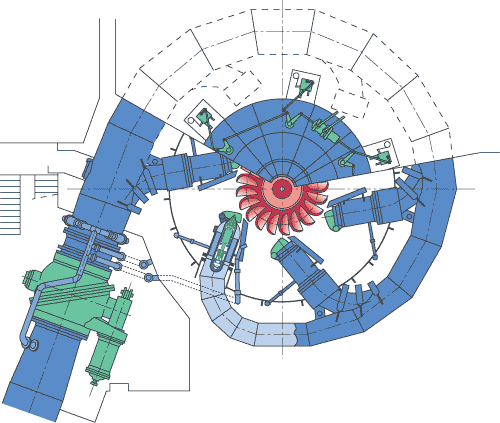
\includegraphics[width = 0.9\textwidth]{report/figures/introduction/pelton.png}
                \caption{Cross section of a Pelton turbine with $6$ needles. By Voith Siemens Hydro Power Generation.\footnote{Licensed under GFDL, Wikimedia Commons \url{https://commons.wikimedia.org/wiki/File:S_vs_pelton_schnitt_1_zoom.png}}} 
                \label{fig:pelton_turbine}
            \end{minipage}
            \hfill\vline\hfill
            \begin{minipage}[b]{0.49\linewidth}
                \centering
                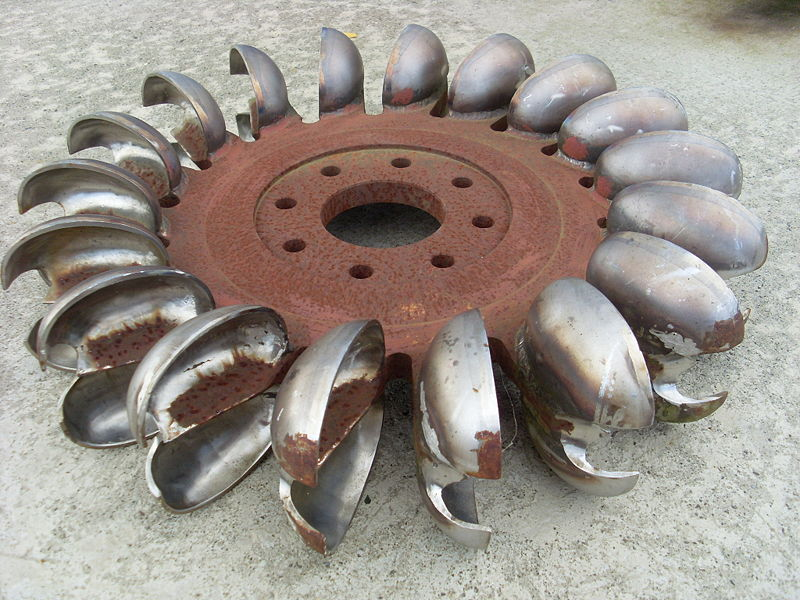
\includegraphics[width = 0.9\textwidth]{report/figures/introduction/pelton_bucket.jpg}
                \caption{A Pelton turbine wheel, the split buckets are easily visible. By Zedh. \footnotetext{Licensed under CC-BY-SA, Wikimedia Commons. \url{https://commons.wikimedia.org/wiki/File:Pelton_400kW_roue_1.JPG}}} 
                \label{fig:pelton_bucket}
            \end{minipage}
        \end{figure}
        
        %!TEX root = ../Thesis.tex
\chapter{Introduction}\label{cha:introduction}
%
% This introductory chapter will briefly provide context for the material/results presented in this report and give motivation and a description of the problem to be solved. A literature review summarizes existing relevant knowledge and establishes the foundation of the later control system. A list of assumptions then defines the scope of the work. Finally, the contributions of the thesis are defined and elaborated.

This is a master thesis written in cooperation between NTNU and Hymatek Controls. Hymatek Controls is located in Oslo and delivers equipment and control systems to hydroelectric power plants worldwide. Hymatek is increasing its focus on condition monitoring and anomaly detection and has acquired a large dataset containing data from a five year period for $27$ hydroelectric power-plants. The goal of this thesis is to find possible use cases for condition monitoring in the provided dataset, research possible techniques and implement some of them in the found use case. Since this is a new research area for Hymatek, this thesis will cover a wide range of aspects. 

This chapter provides an introduction to the work done, describing the motivation and problem description for the thesis. Also, a literature review looking into state of the art techniques used for condition monitoring. Finally, the outline of the report is presented. 


\section{Motivation}\label{sec:motivation}

% % What is the motivation for considering the problems/question that you approach in your work? Why is this an interesting problem? The motivation should instead describe why it is interesting from a societal point of view, and/or from a scientific point of view.

The need for renewable and stable energy sources is great in Norway, Europe and worldwide. According to \cite{Statkraft2009} $99\%$ of the Norwegian power production comes from hydroelectric power plants. Norway has almost $50\%$ of Europe's hydroelectric capacity. Hydroelectric power is one of the most stable and cleanest energy sources one can find \cite{Statkraft2009}. Hydroelectric power plants have a high investment cost, but according to \cite{Selak2014} operation and maintenance costs are as low as 2\% of the cost of the initial investment, this makes it one of the cheapest energy sources one can find. As many European countries are transitioning into renewable energy sources, the need for stable and controllable power sources grows. Both wind and solar power production are dependent on weather conditions, and their production capacity can change quickly and unexpectedly. Norway has been called Europe's renewable battery due to its hydroelectric capacity, and the power delivery capacity is growing. By 2021 Norway and Great Britain will be connected through a new underwater power cable. This example shows that Norway is becoming a part of a more complex energy market. As the exporting capacity grows, green energy from Norway can be supplied to reduce the consumption of fossil energy from for example coal from the European continent. This means that increased productivity and efficiency in hydroelectric power plants effectively can help make the green shift in the European power production happen. 

One way to increase a plant's productivity is to ensure that it is operable at all times. However, this is not possible since one has to perform maintenance on all parts of a plant. Planned maintenance is however not the only reason for a power plant stopping down. Components can breakdown outside of their service interval, leading to unplanned downtime. This is of course not only a case for hydroelectric power plants but more or less any industry or factory. Unplanned downtime is expensive for the energy company that operates the plant, and depending on the time of year and the duration of the breakdown, the cost can have a significant impact on their operation. Finding a way to avoid these breakdowns, and replacing unplanned maintenance with planned maintenance, is something all energy companies find interesting. A hydroelectric power plant contains several large components such as turbines, generators, transformers, hydraulic systems, valves, pipes, and so on.  As an addition comes all the equipment needed to operate the plant. Keeping spare parts for all components would require enormous storage, in addition to tying considerable assets due to the cost of all components. Many components do not need to be often replaced, hence the spare can be left in storage for many years, and may never be replaced. This is not an optimal solution. 

Another approach is to try to eradicate unexpected breakdowns. This means that one needs to have a way to detect that a component is decaying so that one can plan an overhaul or replacement before it breaks down. Eradicating unexpected breakdowns also solves another factor to consider when it comes to breakdowns of components, the domino effect. Depending on the situation and the component, if one component breaks down, it might end up taking several other with it. If a bearing on a turbine shaft breaks down, one risks that the damage will spread to the bearing on the other side of the shaft, and even to the turbine and generator. Continuous analysis of the condition of the bearing could help avoid this issue. This is known as condition monitoring. In its most complete form, condition monitoring gives an insight into the condition of the monitored components, giving an estimate to the remaining lifetime of the component. Introducing condition monitoring could help reduce the number of breakdowns, as components can be replaced before breaking.

There are many good reasons for pursuing the topic of this thesis, on a personal level it is motivating to work with real-world data, to learn the difference between theoretical and practical engineering. Looking for solutions that will improve the operation of a hydroelectric power plant, which can give even more clean energy is also motivating. Additionally, the fact that possible solutions found for the specific cases looked into most likely can be adapted to other industries is also very motivating. 

% An attempt of classifying the wear of the guide vanes on a Francis turbine was performed in my project thesis.  


% This triggered my interest in the possibilities of information found in data. 
% Looking into different possible techniques for condition monitoring that can be utilized on a real-world dataset will give
% As the world becomes more and more digitized, one can either keep up or be left behind. Condition monitoring is seen as an important part of the future portfolio of Hymatek Controls and a necessary addition to continuing their growth into the future. 

% \section{Contributions}
    


\section{Problem definition}

% Korleis oppsto problemstillinga? dreiv å såg gjennom feiloggen etter interesssante feil. Såg då at det var problemer med nålstryinga for hjartdøla. Starta så å undersøke dataen, og fant etterkvart ut at det er 2 anlegg til som har nålstyring. Dei hadde derimot ikkje raportet feil med nålene, noko som gav meg grunn til å tenke at dei har normal oppførsel. Då kunne eg og starte å samanlikne data mellom kraftverka for å sjå kva som er unormal og normal oppførsel.

Hymatek provided no exact problem definition, they provided a dataset containing process-data from $27$ hydroelectric power plants for the period $2013-2017$, and gave no restriction on which plants and cases to investigate. A historical incident log was also provided for all plants, with varying level of detail. Based on this, the problem definition was split into three main parts. As this is a thesis built upon an unknown dataset with unknown quality, an important factor is to recognize what the data can be utilized for, and what improvements that could/ need to be done to make the data analysis more extensive. Ideally, the result of the thesis will be a system for condition monitoring for a real-world case found in the dataset. However, since Hymatek is still in the start-up phase of its condition monitoring research, all experiences from this thesis are valuable. Therefore the most important part of the thesis is to understand why or why not one can create a condition monitoring system for the given case. Then this thesis can be used as a basis for further condition monitoring case analysis. The three parts are as follows: 

\begin{itemize}
    \item Finding techniques and methods for condition monitoring and anomaly detection. Finding methods for feature extraction and dimensionality reduction to be used in addition to the anomaly detection techniques.
    \item Data preparation and case extraction. The provided data is not ready for analysis, and one needs to extract datasets for each of the plants. Once the data is in a format that can be analyzed, the historical data from the plants and the datasets need to be analyzed to build a  case for the further analysis. 
    \item Analyzing the case using the techniques found. Emphasize on how the different techniques perform, and what can/needs to be done to improve the performance. 
\end{itemize}


% \section{Literature review}\label{sec:review}
    

% Start writing about the articles I have already read, can always delete it if it is not relevant in the end. 
%     \subsection{Timeseries forecasting}\label{sec:time_series_forecasting}
    
%     \subsection{One class support vector machine novelty/anomaly detection}\label{sec:ocsvm_novelty_detection}
    
%     \subsection{Neural network novelty/anomaly detection}\label{sec:nn_novelty_detection}
    
%     \subsection{The data set}\label{sec:the_data}
%     The data is provided by Hymatek controls and is collected from more than 30 hydroelectric power plants around Norway, in the period between $01.01.2014$ and $01.07.2017$. 

\section{Limitations}\label{sec:assumptions}
    Since the thesis span over many different research areas, only one case will be analyzed, even if it should be possible to find several more from such an extensive dataset. Also, only a subset of the suggested techniques will be chosen for analysis, spanning from easy to more complex. There might be algorithms not tested that could be useful for the given case. The techniques are chosen in cooperation with Hymatek. 
    
    Availability of computing power and memory also introduces constraints to the analysis. All analysis is performed on a desktop from dell provided by NTNU. This means that no analysis will be performed using the full datasets, they will be reduced by either feature selection or dimensionality reduction. 
    
    Condition monitoring is a broad field, and creating a full-scale condition monitoring system for one case is too comprehensive. The thesis will, therefore, focus on anomaly/novelty detection for the given case. This means that one will train different techniques on normal operation data, and verify how well the different techniques can detect the anomaly found for the specific case. 
    
\section{Hydroelectric power production}\label{ref:sec_hydropower}
    $99\%$ of the Norwegian power production comes from hydroelectric power plants. Hydroelectric power is clean, reliable and once built, it produces cheap energy. \cite{Statkraft2009} claims that no other types of power plants have long expected lifetime and higher efficiency than hydroelectric power. Statkraft also states that countries with the highest increase in energy demand are also countries with the highest unused potential for hydroelectric power. This means that hydroelectric power production can play a significant role in the hunt for meeting the global energy demand. There are many old power plants today, so there are also possibilities for modernization and extensions of already existing plants. 
    
    The principal behind hydroelectric power is simple. It utilizes the energy in running water, converting it to electric energy through a turbine. According to \cite{Paish2002}, there are two main types of turbines, impulse and reaction. The difference between the two types is how they create the rotational force. The impulse turbine rotor runs in air, and the rotational force is created by a water jet lead onto the turbine blades. The reaction turbine is submerged in water, and the rotational force comes from a lift force created by the oncoming water flow. For the impulse turbine, kinetic energy generates the rotational force, for the reaction both kinetic and pressure energy generates it. When the water hits the turbine blades, the water pressure is reduced to atmospheric pressure, and all pressure energy is converted to kinetic energy. For the reaction turbine, which is submerged in water, the water pressure is still high, meaning that one needs a casing which is sealed from atmospheric pressure. 
    
    % \begin{figure}
    %     \centering
    %     \includegraphics{}
    %     \caption{Principal behind reaction and impulse turbines}
    %     \label{fig:my_label}
    % \end{figure}
    
    
    The two most common turbine types are Francis and Pelton. The type used is defined by the size of the flow and the head of the water. Whether the turbine will be producing power only at optimal flow, or if it will be used for power production over a broader range is also a criterion. 
    
    
    
    \subsection{Pelton turbines}\label{subsec:pelton}
        
        The Pelton turbine is the most common impulse turbine. Water is lead onto to the turbine through a series of needles or valves. The turbine has a set of buckets located on the turbine wheel which splits the water jet in two, where each half is deflected back and falls into a discharge channel, \cite{Paish2002}. A cross-section of a Pelton turbine is seen in Figure \ref{fig:pelton_turbine}. As one can see the needles are divided equally around the turbine. The amount of produced power is controlled by the number of active needles, and by regulating their opening. Figure \ref{fig:pelton_bucket} shows how the buckets are designed. Where the water jets hit the buckets is easily verifiable by looking at the corroded parts of the buckets. The needles are controlled by a hydraulic system, which is controlled by the power plant control system. To ensure an even momentum on the turbine, all active needles should have the same opening. 
        
        
        \begin{figure}
            \begin{minipage}[b]{0.49\linewidth}
                \centering
                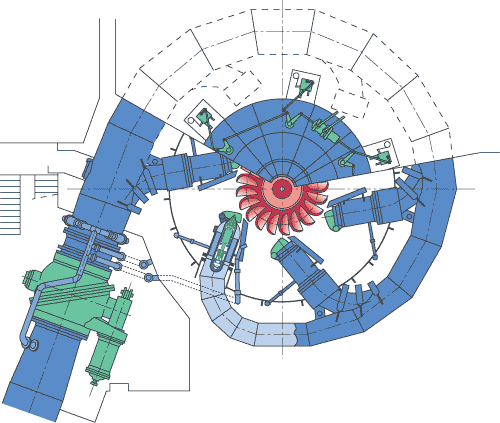
\includegraphics[width = 0.9\textwidth]{report/figures/introduction/pelton.png}
                \caption{Cross section of a Pelton turbine with $6$ needles. By Voith Siemens Hydro Power Generation.\footnote{Licensed under GFDL, Wikimedia Commons \url{https://commons.wikimedia.org/wiki/File:S_vs_pelton_schnitt_1_zoom.png}}} 
                \label{fig:pelton_turbine}
            \end{minipage}
            \hfill\vline\hfill
            \begin{minipage}[b]{0.49\linewidth}
                \centering
                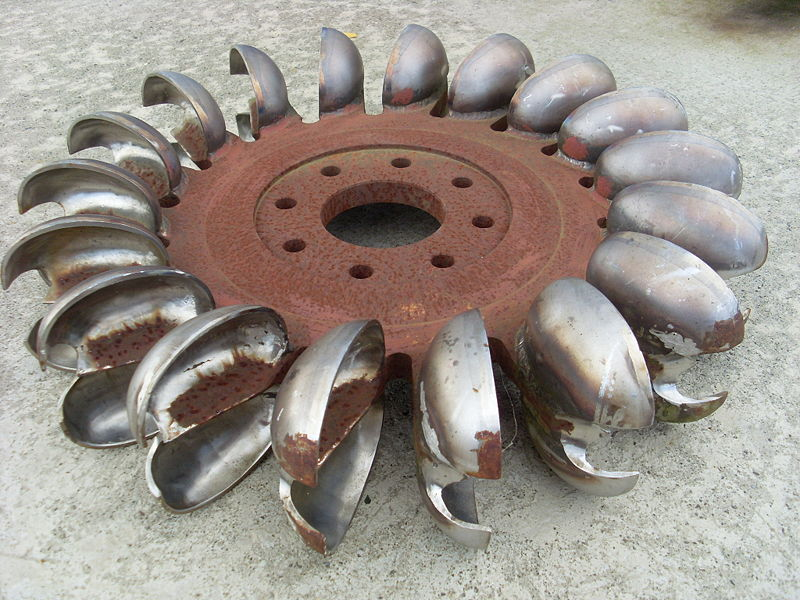
\includegraphics[width = 0.9\textwidth]{report/figures/introduction/pelton_bucket.jpg}
                \caption{A Pelton turbine wheel, the split buckets are easily visible. By Zedh. \footnotetext{Licensed under CC-BY-SA, Wikimedia Commons. \url{https://commons.wikimedia.org/wiki/File:Pelton_400kW_roue_1.JPG}}} 
                \label{fig:pelton_bucket}
            \end{minipage}
        \end{figure}
        
        
    
    \subsection{Francis turbines}\label{subsec:francis}
        The Francis turbine is a reaction turbine. The water is lead onto the turbine through a set of guide vanes connected to the spiral casing, and lead out from the center of the turbine. The guide vanes control the amount of water lead to the turbine, and hence the amount of produced energy. A cross-section of a Francis turbine is seen in Figure \ref{fig:francis}. All guide vanes have the same opening and are controlled through a ring mounted on the top of the turbine. Figure \ref{fig:guide_vanes} shows a hydraulic actuator used to control the ring that operates the guide vanes. As for the Pelton turbine, the hydraulics is again controlled by the plant's control system. \cite{Aasnes2017} tries to classify the condition of the guide vanes in a Francis turbine using different machine learning methods such as support vector machines (SVM), neural networks (NN) and regression.   
        
        \begin{figure}
            \begin{minipage}[b]{0.49\linewidth}
                \centering
                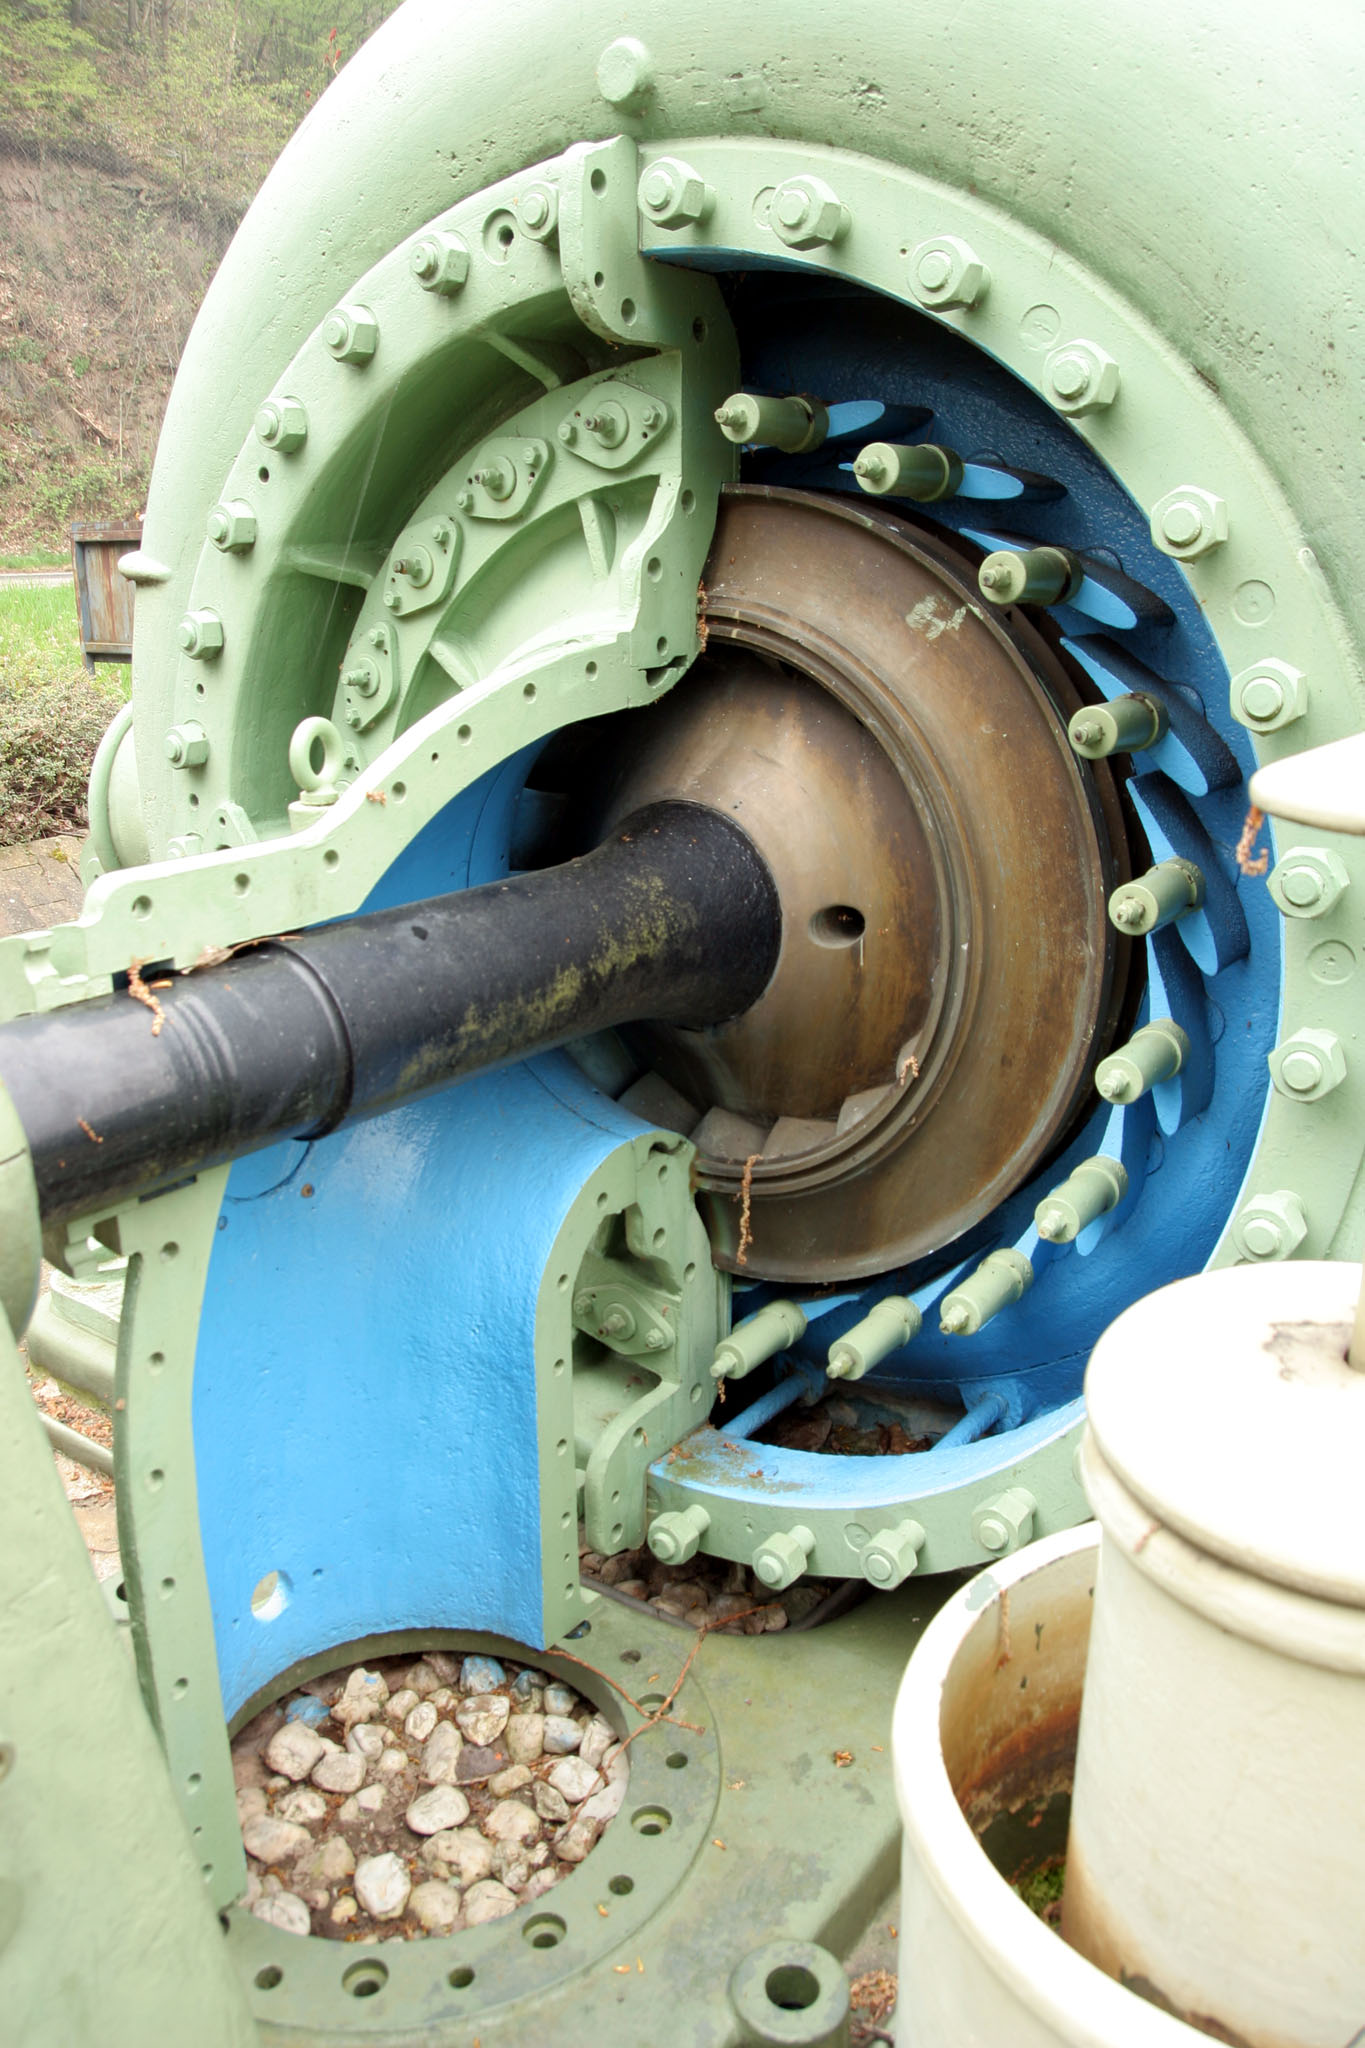
\includegraphics[width = 0.9\textwidth]{report/figures/introduction/francis_turbine.jpg}
                \caption{Cross section of a Francis turbine. The guide vanes are seen in almost closed position. By Armin Kübelbeck.\footnote{Licensed under CC-BY-SA, Wikimedia Commons, \url{https://commons.wikimedia.org/wiki/File:Fankel_Francisturbine_01.jpg}}}
                \label{fig:francis}
            \end{minipage}
            \hfill\vline\hfill
            \begin{minipage}[b]{0.49\linewidth}
                \centering
                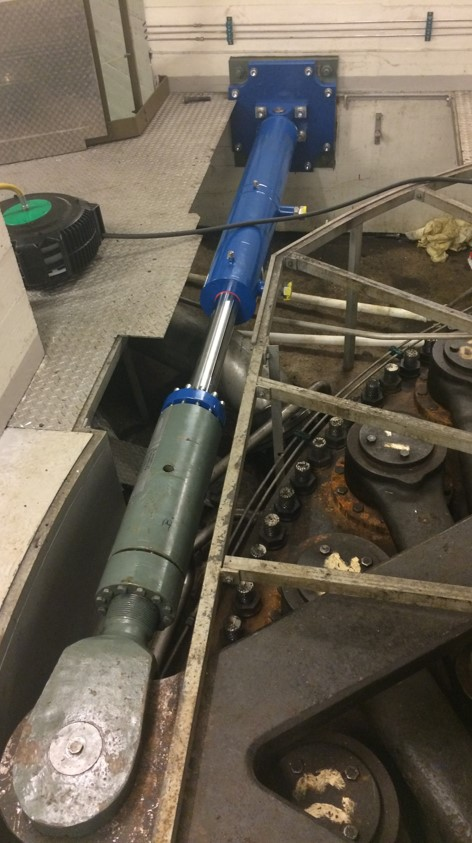
\includegraphics[width = 0.9\textwidth]{report/figures/introduction/servo1(1).jpg}
                \caption{Hydraulic actuator for guide vane control. The actuator is mounted to a ring that controls the guide vane opening. Courtesy of Hymatek Controls}
                \label{fig:guide_vanes}
            \end{minipage}
        \end{figure}
        
    \subsection{Other equipment}
        There are several other large components in a hydro-electrical power plant. Among them are;
        \begin{itemize}
            \item Generators
            \item Transformers
            \item Coolers
            \item Hydraulic systems
        \end{itemize}
    
    \section{Condition monitoring for hydroelectric power plants}\label{sec:cm}
        \cite{Selak2014} presents a complete condition monitoring and fault detection system for hydroelectric power plants, covering everything from data acquisition to fault detection methods. Cost reduction, increase in equipment availability and increased performance are presented as the benefits of introducing condition monitoring. They propose using condition monitoring in addition to preventive maintenance and claim that it is the most comprehensive maintenance scheme available. Data is transferred to a virtual diagnostics center, where an SVM is used to diagnose the data. The proposed condition monitoring system is separated into six steps; data acquisition, data analysis and storage, data transferring, data selection, SVM training and SVM testing. It is proposed to sample data in four different ways to reduce the amount of data stored; periodically at a predefined sampling rate, when signal values exceed a threshold, during transients and sudden events. 
        
        Using SVM for fault diagnostics, data that represents all known failure modes, in addition to normal data is needed. This has restricted the work only to include two variables at a time, as this enables scatterplotting variables against each other for visual confirmation of the normal operation. The training cases separate data into four different datasets; All input data, removing low power operations, removing high water flow operations and removing transients between operation regimes. Experts extracted 44 causalities that can be traced to a pair of process variables. Abnormal data is created as a complement to the normal data, by fitting an oversized boundary to the data from normal operation. As the SVM detector is only trained on two classes, data is only evaluated as normal or abnormal. It is claimed that two-dimensional models are sufficient to catch all known failure modes. The choice of using SVM is supported by \cite{Widodo2007} that presents that SVM has been successfully used in the industry for several different use-cases. 
        
        \cite{Molina2000} introduces two NN approaches to integrate into a decision system for hydroelectric power plant management. An expert system, an NN for acoustic prediction and an NN for predictive maintenance are proposed integrated into one system. It is argued that there are non-linear plant dependencies undetectable for a human expert, that the NN can find. As the expert system tries to mimic the response of a human operator, the system suffers from the same limitations as a human operator. Interpreting an expert system is however much more straightforward than interpreting an NN. Therefore a hybrid system is proposed, benefiting from the best of both worlds. The expert system and the NN for predictive maintenance relay on process data from the plant. The NN for acoustic prediction is fed with data recorded from sensors not used in the two other cases. 106 process variables are available for analysis, all are given as input to the NN, but to mimic the limitations of a human operator, the expert system is only considering 15 variables at a time. The NN for predictive maintenance needs data that represent both normal and abnormal data, for all known failure modes. A particular procedure combining expert knowledge and NNs are used to create data vectors with values for all 106 variables for the given errors created by the expert system. Once the error vectors are created, those are used to train the NN. Classes for the acoustic prediction network were created based on an experts classification of the normal and abnormal regime based on the plants generated power. 
        
        The proposed method was applied and test on a plant in Zamora, Spain. It was found that the combination of the NNs and the expert system outperformed a human operator, but the human operator outperformed the methods individually. The NN for predictive maintenance gave the best individual results. The NN for acoustic predictions suffered from variability in the acoustic signals, but showed that it served as a good addition to the two other methods. 
        
        
    
    
    
    \section{Report outline}
    Chapter \ref{cha:litterature} introduces different anomaly detection techniques, and methods for feature selection and dimensionallity. Chapter \ref{cha:implementation} introduces the software and the libraries used in this thesis. Chapter \ref{cha:data} introduces the dataset and the cases analyzed. Chapter \ref{cha:analysis} walks the reader through the analysis before the discussion and conclusion are found in chapters  \ref{cha:discussion} and \ref{cha:conclusions}.  
% \section{Background and Contributions}\label{sec:contributions}
% Here you describe the main contributions of your project work: What are the new results - the achievements - of your work. 

% It is important that you here also clearly describe which background material you have received. Which information, software, equipment etc. have been made available for you, or form the basis for your work. Which help and support have you received, and from who, during your work. For instance: The Matlab simulator used in Section 2 was provided to me by Ph.D. candidate NN, and I have adapted this to the problem in this thesis by modifying...

% \section{Outline}\label{sec:outline}
% The report is organized as follows. In Chapter~\ref{cha:first} a mathematical model is developed to describe the system... In Chapter

    
    \subsection{Francis turbines}\label{subsec:francis}
        The Francis turbine is a reaction turbine. The water is lead onto the turbine through a set of guide vanes connected to the spiral casing, and lead out from the center of the turbine. The guide vanes control the amount of water lead to the turbine, and hence the amount of produced energy. A cross-section of a Francis turbine is seen in Figure \ref{fig:francis}. All guide vanes have the same opening and are controlled through a ring mounted on the top of the turbine. Figure \ref{fig:guide_vanes} shows a hydraulic actuator used to control the ring that operates the guide vanes. As for the Pelton turbine, the hydraulics is again controlled by the plant's control system. \cite{Aasnes2017} tries to classify the condition of the guide vanes in a Francis turbine using different machine learning methods such as support vector machines (SVM), neural networks (NN) and regression.   
        
        \begin{figure}
            \begin{minipage}[b]{0.49\linewidth}
                \centering
                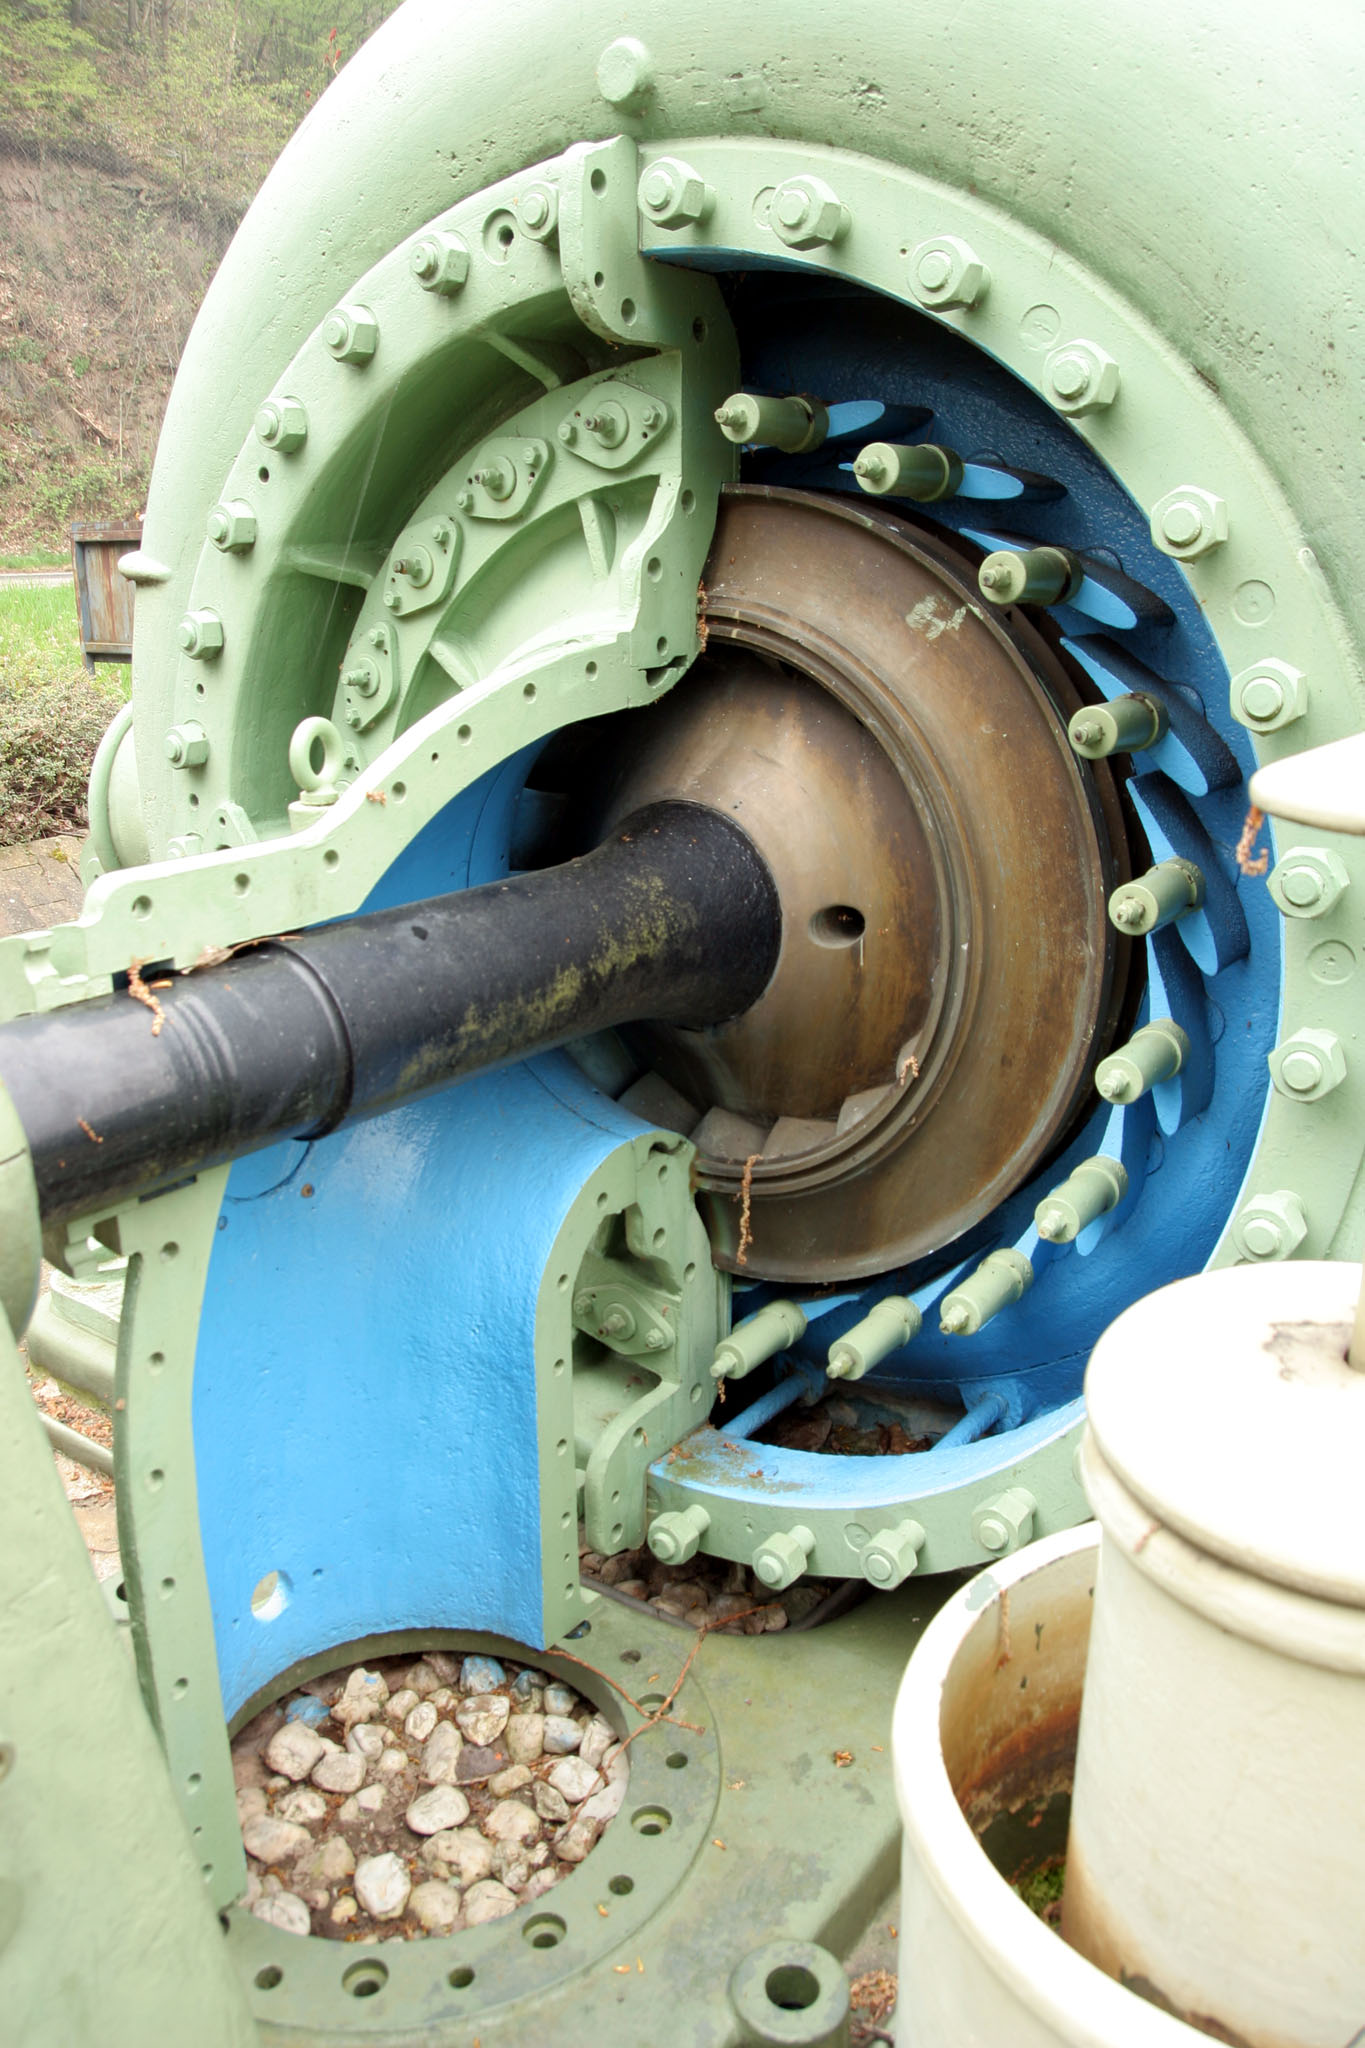
\includegraphics[width = 0.9\textwidth]{report/figures/introduction/francis_turbine.jpg}
                \caption{Cross section of a Francis turbine. The guide vanes are seen in almost closed position. By Armin Kübelbeck.\footnote{Licensed under CC-BY-SA, Wikimedia Commons, \url{https://commons.wikimedia.org/wiki/File:Fankel_Francisturbine_01.jpg}}}
                \label{fig:francis}
            \end{minipage}
            \hfill\vline\hfill
            \begin{minipage}[b]{0.49\linewidth}
                \centering
                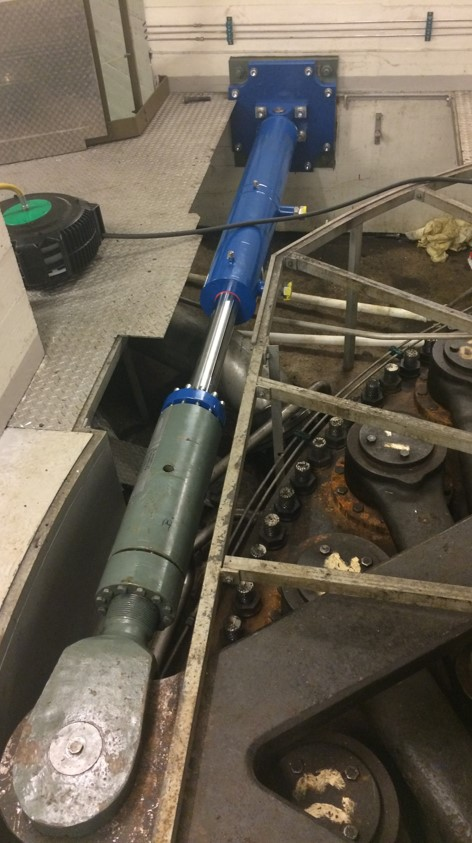
\includegraphics[width = 0.9\textwidth]{report/figures/introduction/servo1(1).jpg}
                \caption{Hydraulic actuator for guide vane control. The actuator is mounted to a ring that controls the guide vane opening. Courtesy of Hymatek Controls}
                \label{fig:guide_vanes}
            \end{minipage}
        \end{figure}
        
    \subsection{Other equipment}
        There are several other large components in a hydro-electrical power plant. Among them are;
        \begin{itemize}
            \item Generators
            \item Transformers
            \item Coolers
            \item Hydraulic systems
        \end{itemize}
    
    \section{Condition monitoring for hydroelectric power plants}\label{sec:cm}
        \cite{Selak2014} presents a complete condition monitoring and fault detection system for hydroelectric power plants, covering everything from data acquisition to fault detection methods. Cost reduction, increase in equipment availability and increased performance are presented as the benefits of introducing condition monitoring. They propose using condition monitoring in addition to preventive maintenance and claim that it is the most comprehensive maintenance scheme available. Data is transferred to a virtual diagnostics center, where a SVM is used to diagnose the data. The proposed condition monitoring system is separated into six steps; data acquisition, data analysis and storage, data transferring, data selection, SVM training and SVM testing. It is proposed to sample data in four different ways to reduce the amount of data stored; periodically at a predefined sampling rate, when signal values exceed a threshold, during transients and during sudden events. 
        
        Using SVM for fault diagnostics, data that represents all known failure modes, in addition to normal data is needed. This has restricted the work to only include two variables at a time, as this enables scatterplotting variables against each other for visual confirmation of the normal operation. The training cases separate data into four different datasets; All input data, removing low power operations, removing high water flow operations and removing transients between operation regimes. Experts extracted 44 causalities that can be traced to a pair of process variables. Abnormal data is created as a complement to the normal data, by fitting an oversized boundary to the data from normal operation. As the SVM detector is only trained on two classes, data is only evaluated as normal or abnormal. It is claimed that two-dimensional models are sufficient to catch all known failure modes. The choice of using SVM is supported by \cite{Widodo2007} that presents that SVM has been successfully used in the industry for several different use-cases. 
        
        \cite{Molina2000} introduces two NN approaches to integrate into a decision system for hydroelectric power plant management. An expert system, a NN for acoustic prediction and a NN for predictive maintenance are proposed integrated into one system. It is argued that there are non-linear plant dependencies undetectable for a human expert, that the NN can find. As the expert system tries to mimic the response of a human operator the system suffers from the same limitations as a human operator. Interpreting an expert system is however much easier than interpreting a NN, therefore a hybrid system is proposed, benefiting from the best of both worlds. The expert system and the NN for predictive maintenance relay on process data from the plant. The NN for acoustic prediction is fed with data recorded from sensors not used in the two other cases. 106 process variables are available for analysis, all are given as input to the NN, but to mimic the limitations of a human operator, the expert system is only considering 15 variables at a time. The NN for predictive maintenance needs data that represent both normal and abnormal data, for all known failure modes. A special procedure combining expert knowledge and NNs are used to create data vectors with values for all 106 variables for the given errors created by the expert system. Once the error vectors are created, those are used to train the NN. Classes for the acoustic prediction network were created based on an experts classification of the normal and abnormal regime based on the plants generated power. 
        
        The proposed method was applied and test on a plant in Zamora, Spain. It was found that the combination of the NNs and the expert system outperformed a human operator, but the human operator outperformed the methods individually. The NN for predictive maintenance gave the best individual results. The NN for acoustic predictions suffered from variability in the acoustic signals, but showed that it served as a good addition to the two other methods. 
        
        
    
    
    
    \section{Report outline}
    Chapter \ref{cha:litterature} introduces different anomaly detection techniques, and methods for feature selection and dimensionallity. Chapter \ref{cha:implementation} introduces the software and the libraries used in this thesis. Chapter \ref{cha:data} introduces the dataset and the cases analyzed. Chapter \ref{cha:analysis} walks the reader through the analysis before the discussion and conclusion are found in chapters  \ref{cha:discussion} and \ref{cha:conclusions}.  
% \section{Background and Contributions}\label{sec:contributions}
% Here you describe the main contributions of your project work: What are the new results - the achievements - of your work. 

% It is important that you here also clearly describe which background material you have received. Which information, software, equipment etc. have been made available for you, or form the basis for your work. Which help and support have you received, and from who, during your work. For instance: The Matlab simulator used in Section 2 was provided to me by Ph.D. candidate NN, and I have adapted this to the problem in this thesis by modifying...

% \section{Outline}\label{sec:outline}
% The report is organized as follows. In Chapter~\ref{cha:first} a mathematical model is developed to describe the system... In Chapter

% \chapter{Data and power plants}\label{cha:data}
% %!TEX root = ../Thesis.tex
\chapter{Cases}\label{cha:cases}
This chapter introduces the different cases this thesis looks into. 

\section{Pelton needles}\label{sub:pelton_needles}
    As mentioned, there was data available from two different power plants with pelton turbines controlled in a similar maner. One of plants had recorded several issues with the needle control, and was used as a case to test early detection of problems with the needle operation. 
    
    \begin{figure}
        \centering
        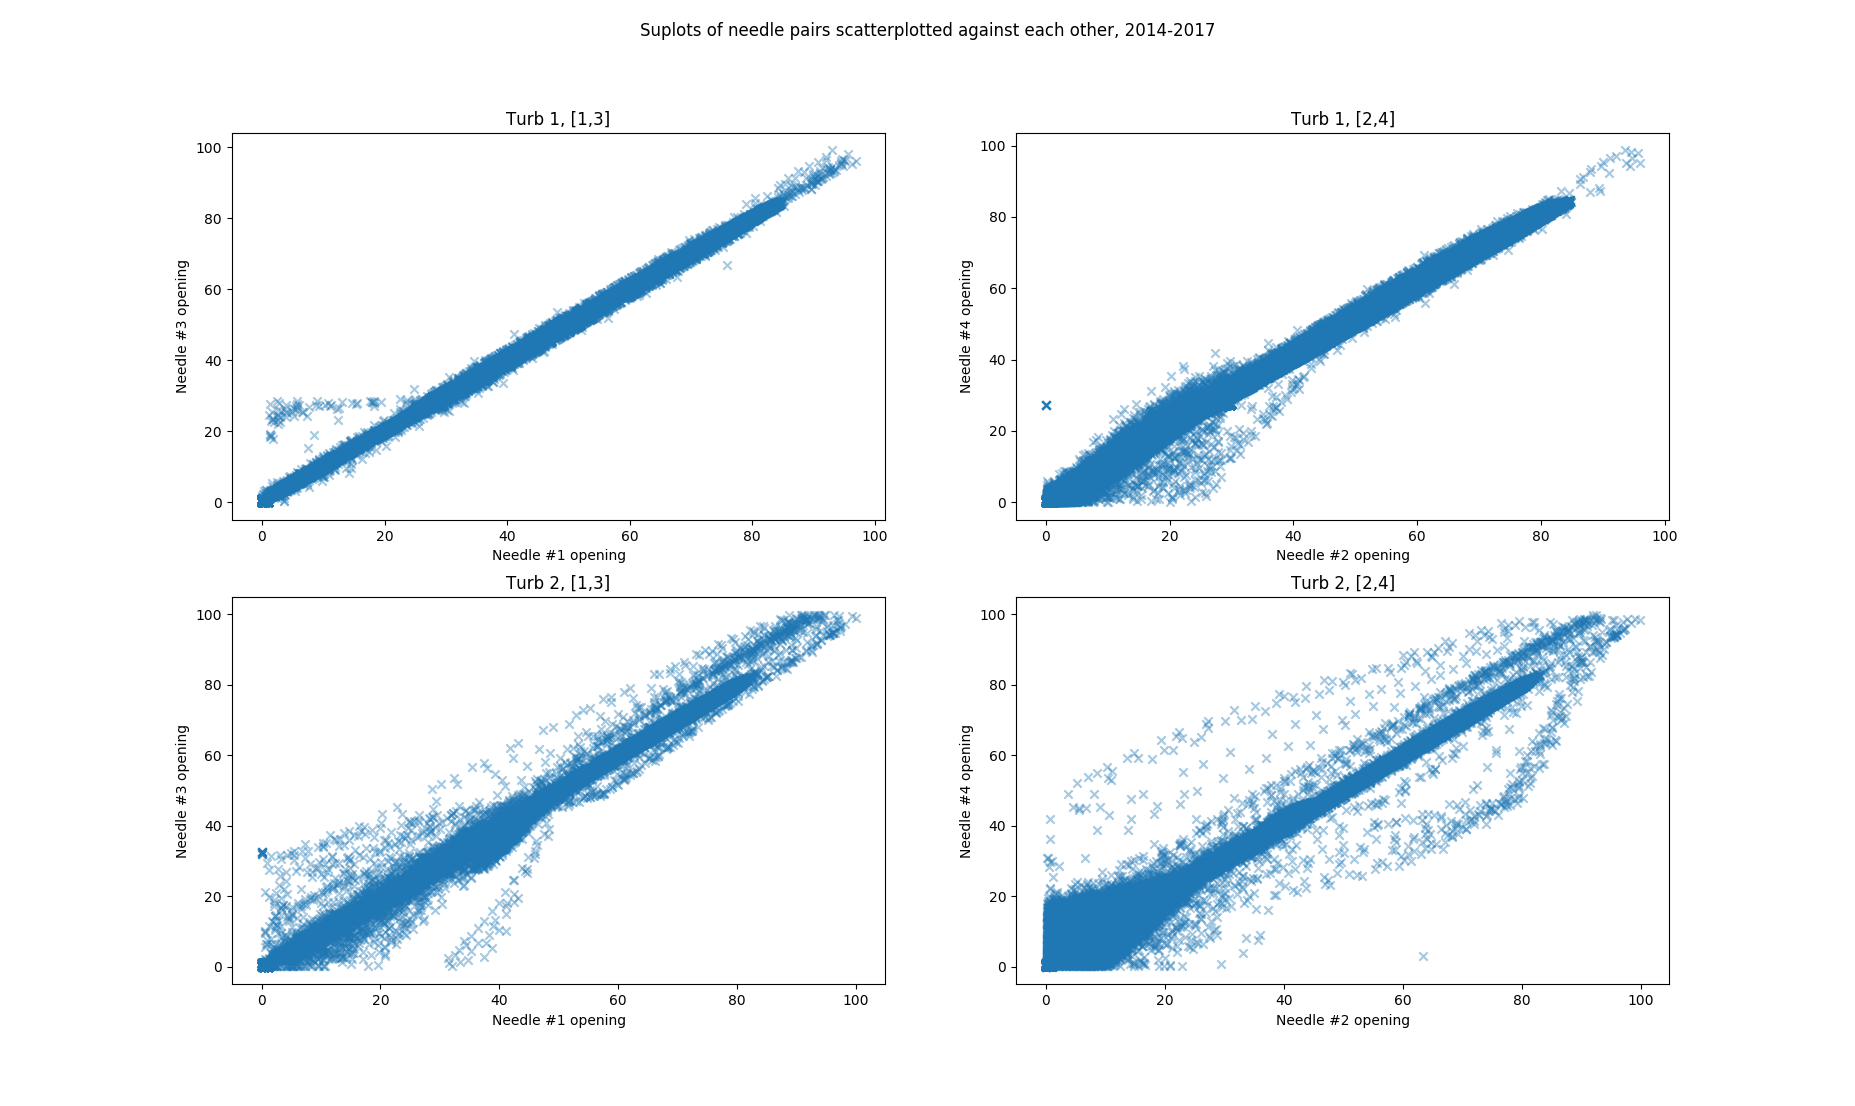
\includegraphics[width=\textwidth]{report/figures/analysis/hjartdola/hjar_scatterplot_all_needels.png}
        \caption{Caption}
        \label{fig:my_label}
    \end{figure}
    
    
    \begin{figure}
        \centering
        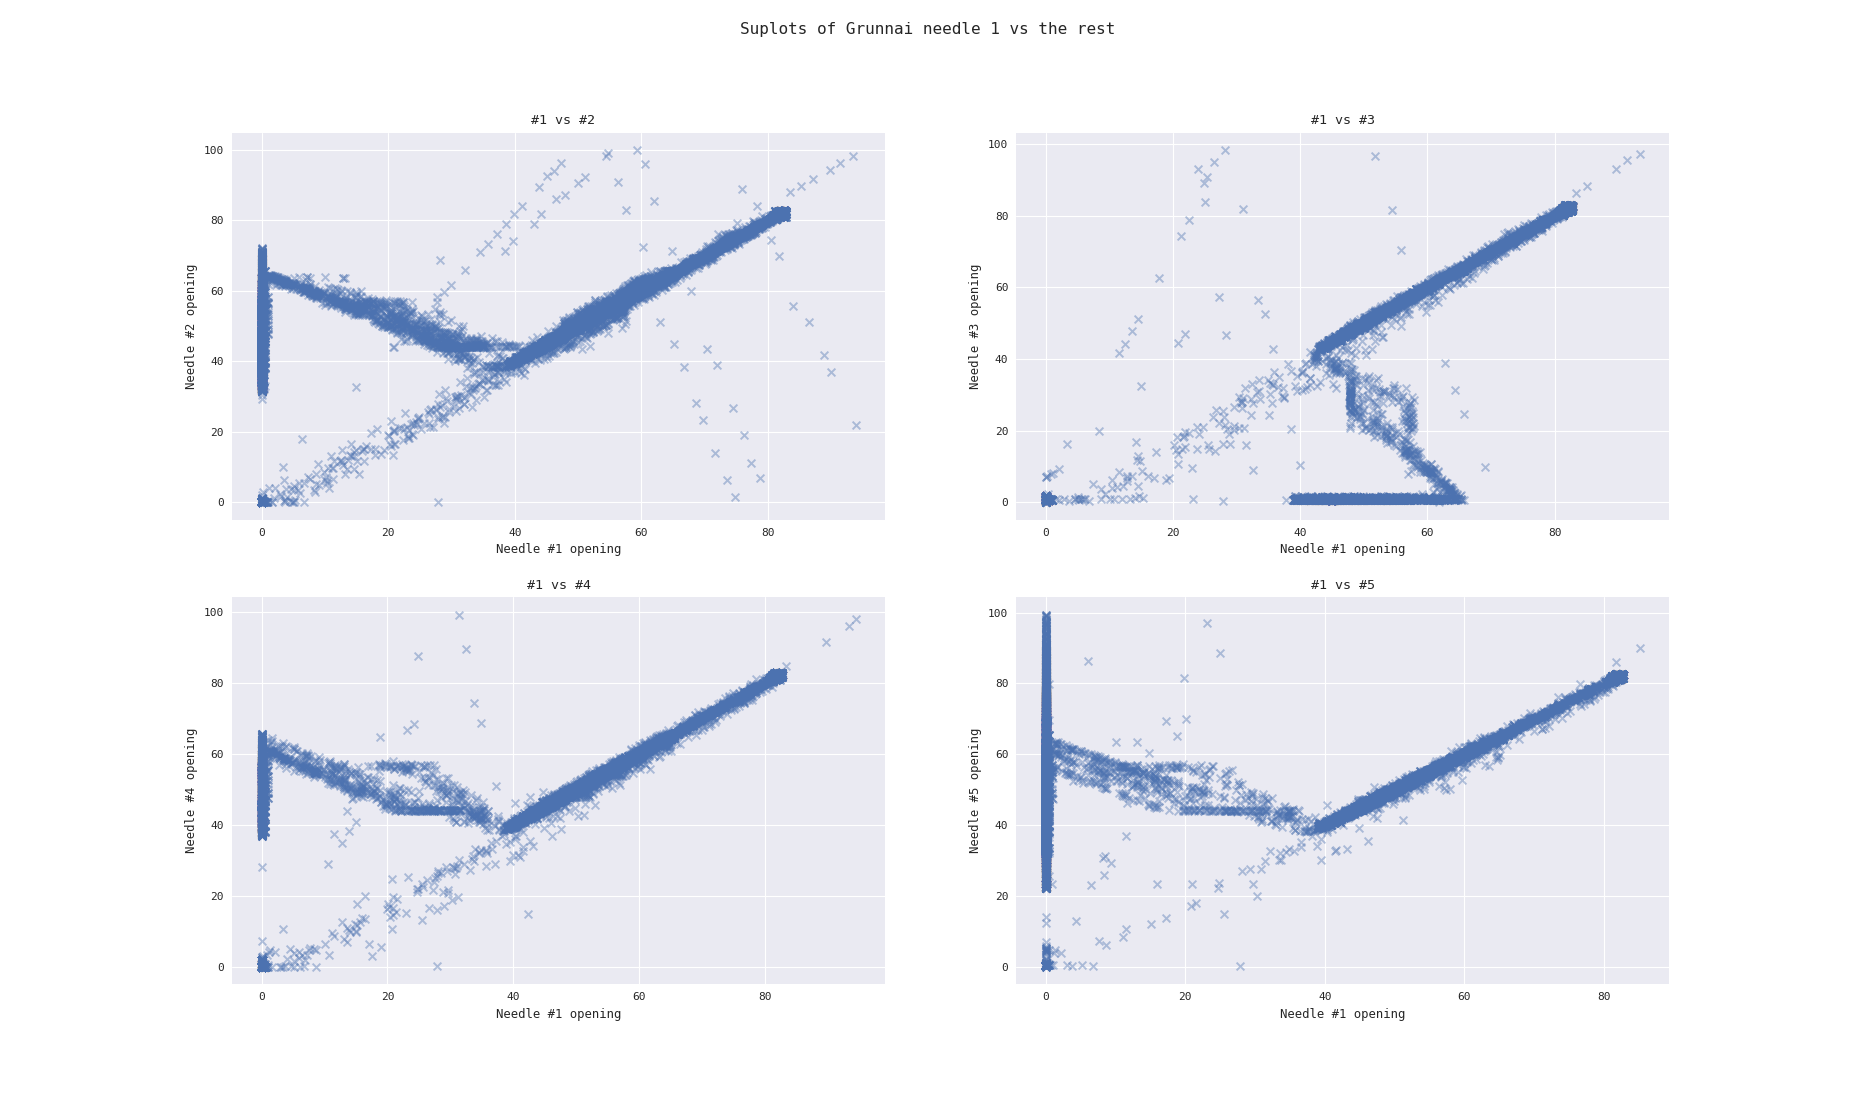
\includegraphics[width=\textwidth]{report/figures/analysis/grunnai/grun_scatterplot_1_vs_rest.png}
        \caption{Caption}
        \label{fig:my_label}
    \end{figure}
    
    
    \begin{figure}
        \centering
        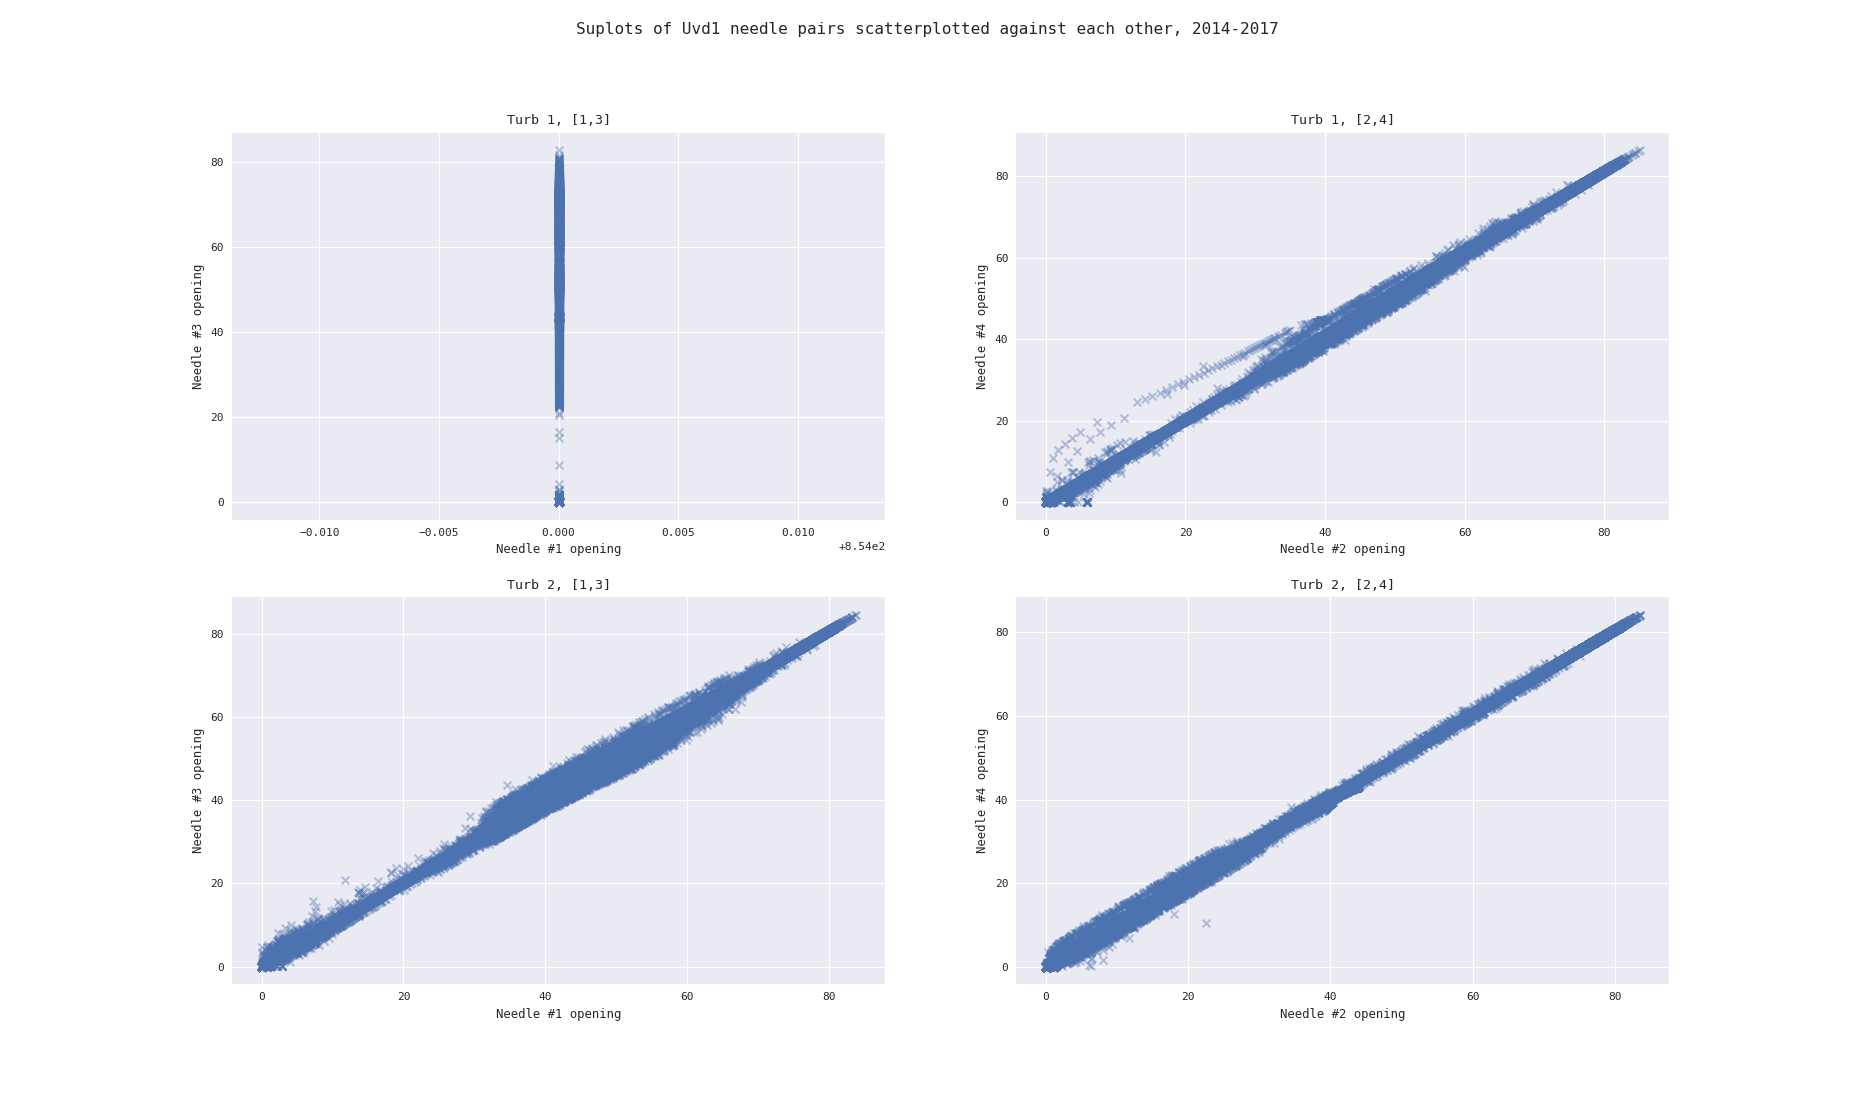
\includegraphics[width=\textwidth]{report/figures/analysis/uvdal1/uvd1_scatterplot_all_needels.png}
        \caption{Caption}
        \label{fig:my_label}
    \end{figure}
    

% \chapter{Techniques}\label{chap:techniques}

Reduction of the number of features in the data is desirable, firstly it simplifies the model, makin it computationally faster. Secondly, a simpler model is easier to interpret. A good understadning of how and why an algorithm behaves as it does is important! There are two main techniques for reducing the feature size, feature selection, and dimensionality reduction. The former, removes uninformative and redundant features from the feature set. The latter creates new features either as linear or non-linear combinations of the original feature set.

\section{Feature selection}\label{sec:feature_selec}

    \subsection{}

\section{Dimensionality reduction}\label{sec:dim_red}
The dimensions of the new set is then often decied by how much the new features explain of the variance in the old dataset. 
    \subsection{PCA}\label{subsec:PCA}
    
    \subsection{Kernel PCA}\label{subsec:kernelPCA}


\section{Anomaly detction}\label{sec:Anomaly_detection}
    
    \subsection{One class SVM}\label{subsec:OCSVM}
    
    \subsection{Neural Networks}\label{subsec:NN}
    
    \subsection{K-nearest neigbours}\label{subsec:k_neig}
    
    \subsection{K-means clustering}\label{subsec:k_means}
    
% %!TEX root = ../Thesis.tex
\chapter{Analysis}\label{cha:analysis}
This chapter contains the anomaly detection analysis performed on the data presented in \ref{sec:pelton_needles}. The goal is to investigate how well different methods detect anomalies when only being exposed to normal data during training. Three anomaly detection techniques are used, one class support vector machine, kernel density estimation, and long short-term memory recurrent neural network. First, the different cases analyzed are presented, then some prepossessing steps are introduced before the optimal hyperparameters of the different methods are presented. Finally, the performance of the different methods on the different cases is presented and compared.

    \section{Cases}
        Due to the aperiodic sampling of process signals, only the needle positions are sampled often enough to be included as features in the analysis. This means that the techniques for feature and dimensionality reduction presented in chapter \ref{cha:litterature} will not be used. The anomaly detection techniques are trained on three different training sets and evaluated on two test sets, production data from plant 1 turbine 2 and the artificial error created on data from plant 2 turbine 2. The goal is to analyze how the methods evaluate the two different cases, to see if they are able to detect the trends seen in chapter \ref{cha:data}. The artificial case enables one to evaluate how early the methods detect anomalies when knowing exactly the start date of the system degradation. 
        
        The three different training sets are presented in table \ref{tab:training_cases}. There are two training sets from plant 2 that only differ in size. This is done to evaluate if the performance of the anomaly detection techniques changes when exposed to more or less data. Training set 1 is the data from plant 1 turbine 2 after the reported incident when the needle operation is back to normal. To ensure that one is not overfitting the techniques on the training data it is important to separate the data into training and validation sets. There is no one golden rule for the ratio between testing and validation, but according to \cite{Kohavi1995} somewhere around $1/3$ of the data is common to use for validation. Only seven months of data is available from plant 1 turbine 2 after the needles are fixed. Therefore five months are used as training data and little under two months for validation. This resulted in a training set of 9449 samples. To enable a comparison between the techniques for different training set sizes, the data from plant 2 is split into two different training sizes. One which is approximate of the same size as training set 1 and one which is approximately ten times larger. 

        Table \ref{tab:test_cases} shows the two test cases. The first case is all data not used for training and validation from plant 1 turbine 2 needle pair [2,4]. As this is the needle pair with the recorded incident, it is interesting to see how the different methods evaluate the data, especially building up towards the reported incident. Case 2 is the artificial case introduced in \ref{subsec:arti}.
        
        
        Training and evaluating the methods on data from two plants enables one to evaluate cross plant performance. This is very interesting, if it can be shown that one can simply deploy a pre-trained anomaly detection system at new plants with little to no alteration, this will greatly reduce the cost of installing such systems. 
        \begin{table}[]
            \centering
            \begin{tabular}{|c|c|c|c|c|c|}
                \hline
                Set    & Plant & Needle pair   & Train             & Validation        & Training samples\\ \hline
                1       & 1     & 2,4           & 20170304-20170701 & 20170701-20170825 & 9449\\ \hline
                2       & 2     & 2,4           & 20160422-20160506 & 20160506-20170101 & 12870\\ \hline
                3       & 2     & 2,4           & 20160101-20160506 & 20160506-20170101 & 84263\\ \hline
            \end{tabular}
            \caption{Table over the three different training cases}
            \label{tab:training_cases}
        \end{table}
        
        \begin{table}[]
            \centering
            \begin{tabular}{|c|c|c|c|c|c|}
                \hline
                Case    & Plant & Needle pair   & Testing               \\ \hline
                1       & 1     & 2,4           & 20140101-20170304     \\ \hline
                2       & 2     & 2,4           & 20161001-20170401     \\ \hline
            \end{tabular}
            \caption{Table over the two different test cases}
            \label{tab:test_cases}
        \end{table}
        
        
        
    \section{Prepossessing steps}
        The data needs to be preprocessed before it can be analyzed. First, all time steps where not both needles are sampled are removed. Secondly, \cite{Tarassenko2009} talks about the importance of removing steady-state samples from the dataset, to avoid biasing the data.  The needles are constantly changing during operation, hence the only steady state is when the plant is not operating. Steady state is removed by removing all samples where the process signal values are close to zero ($<2$) and unchanged since the last sample. Having a stationary time series is important. As \cite{Manuca1996} explains, many of the common techniques for analyzing time series assume that the given series is stationary. A stationary time series is said to be independent of time, and don't have any correlations with seasonality. As all no operation data is removed from this dataset, the data is seen as stationary. The next step is to scale the data. For SVM and KDE, the data is scaled to zero mean and unit variance, for the LSTM RNN the data is scaled within a range of [0,1]. This was found to yield the optimal behavior for the different algorithms. To enable cross testing between plants, the transformations are calculated on plant 1 turbine 2 needles [2,4] and used for all datasets. Finally, the data is checked for outliers using scatterplots, as having anomalies in the training data could damage the systems ability to detect anomalies. 
    
    \section{Hyperparameterization}
        The methods chosen for the anomaly detection have several different parameters or hyperparameters. To ensure that the methods perform optimally, it is necessary to search for the best combination of these parameters. To enable a reasonable comparison between the different cases analyzed, an optimal parameterization is found and used for all cases. 
            \subsection{One class support vector machine}
                The one class SVM has two tunable parameters. These are $\gamma$ and $\nu$. There is, however, no good way to automatically find the optimal parameterization for unlabeled data. The cases presented in this thesis have no labeled data. By default, one has to manually inspect the one class SVM performance for different hyperparameterizations. An attempt to create a custom cost function that could be used for automatic hyperparameterization is made. The cost function is built upon the idea that a good separating hyperplane or decision boundary lay close to the samples. The one class SVM implementation in scikit learn gives the signed distance from each sample to the separating hyperplane. This can be used to evaluate the shape of the decision boundary. The proposed cost function is seen in equation \ref{eq:svm_cost} where $\bm{x}$ is the vector with the signed distances for each sample to the separating hyperplane. Several different setups for a cost function were tried. The chosen performed well for the cases studied in this thesis. One cannot guarantee that it will perform adequately for different cases.  
                
                \begin{align}
                    \score = 1 - \abs(\std(\bm{x})) - \abs(\mean(\bm{x})) -\frac{\outliers}{\inliers}100
                    \label{eq:svm_cost}
                \end{align}
            
                As explained in the theory, $\nu$ can be interpreted as an upper boundary for the fraction of outliers. Since the data is assumed to be outlier free, it is natural to pick values for $\nu$ that lie around $\frac{1}{N}$ where $N$ is the number of samples. $\gamma$ is a measure of the complexity of the decision boundary and is therefore chosen to span a wide range of values. A grid search is performed over the values seen in the list below. 
                \begin{itemize}
                    \item $\gamma =  [0.01,0.05,0.1,0.2,0.4,0.8,1,2,4,8,16]$
                    \item $\nu = [\frac{1}{25N}, \frac{1}{10N},\frac{1}{5N},\frac{1}{2N},\frac{1}{N},\frac{2}{N},\frac{5}{N},\frac{10}{N}]$
                    \label{list:svm_grid}
                \end{itemize}
                Table \ref{tab:svm_gridsearch} shows the score and parameterization for the five best and five worst combinations. Figure \ref{fig:svm_grid_best} shows the decision boundary for the classifier that scored the best with regards of the cost function defined in equation \ref{eq:svm_cost}. The boundary covers all samples with a reasonable distance from the samples. As can be seen, most of the support vectors are located at the upper and lower range of the samples, showing the importance of having training data that span the full operating range of the machinery. A couple of samples in the mid area are also picked as support vectors, this gives a relatively close, but smooth boundary. The boundary for the worst parameterization is seen in figure \ref{fig:svm_grid_wors}, it is easily verified that the boundary is to complex, due to a large $\gamma$ and a very small $\nu$. The decision boundaries for the remaining classifiers are found in appendix \ref{apendix:svm_grid}. it can be verified that all of the high scoring classifiers have a similar shape of the decision boundary. Note that the plots are produced using the scaled data. 
                
                
                
                \begin{table}[h]
                    \centering
                    \begin{tabular}{|c|c|c|}
                        \hline
                         Score  &   $\gamma$    & $\nu$         \\ \hline
                         0.975  &   $0.05$      & $\frac{1}{N}$ \\ \hline
                         0.970  &   $0.1$      & $\frac{1}{2N}$ \\ \hline
                         0.961  &   $0.1$      & $\frac{1}{N}$ \\ \hline
                         0.960  &   $0.05$      & $\frac{2}{N}$ \\ \hline
                         0.957  &   $0.2$       & $\frac{1}{N}$ \\ \hline
                         -44.437  &   $8$      & $\frac{1}{10N}$ \\ \hline
                         -51.780  &   $8$      & $\frac{1}{25N}$ \\ \hline
                         -57.461  &   $0.1$      & $\frac{1}{25N}$ \\ \hline
                         -71.082  &   $16$      & $\frac{1}{10N}$ \\ \hline
                         -506.263  &   $16$      & $\frac{1}{25N}$ \\ \hline
                         
                    \end{tabular}
                    \caption{Table showing the five best and five worst scores for the gridsearch after optimal hyperparameters for the one class SVM. $N = $ number of samples.}
                    \label{tab:svm_gridsearch}
                \end{table}
                
                \begin{figure}
                        \centering
                        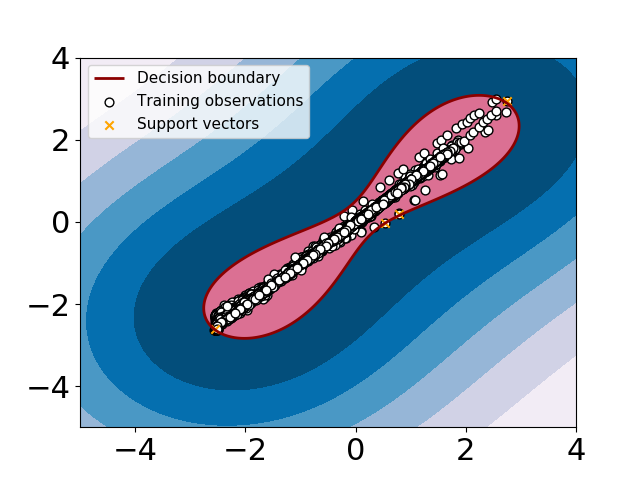
\includegraphics[width=0.7\textwidth]{report/figures/analysis/gridsearch/Novelty detection, 1, training, gamma = 0.05 nu = 1.0583130489998942e-05.png}
                        \caption{Decision boundary found for the best scoring classifier}
                        \label{fig:svm_grid_best}
                        
                \end{figure}
                
                \begin{figure}
                        \centering
                        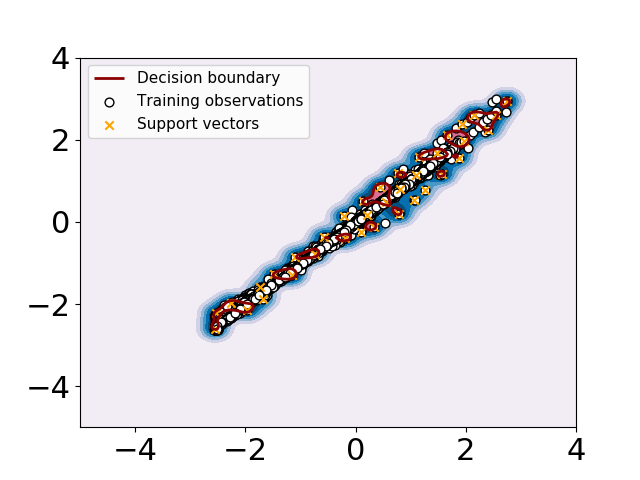
\includegraphics[width=0.7\textwidth]{report/figures/analysis/gridsearch/Novelty detection, -1 training, gamma = 16 nu = 4.233252195999577e-06.png}
                        \caption{Decision boundary for the worst classifier}
                        \label{fig:svm_grid_wors}
                \end{figure}
    
                
                
            \subsection{Kernel density estimation}
                The optimal hyperparameters for KDE were found using the built-in grid search method in scikit-learn. The different parameterizations are scored based on how well they replicate the distribution of the original data. As with one class SVM, KDE only has two parameters, bandwidth and kernel type. The bandwidth serves as a smoothing parameter, the higher the bandwidth the smoother the density estimation will become. The KDE grid search was performed over a bandwidth from $[0,1]$ at $0.1$ steps, and with Gaussian, Tophat, Epanechnikov, Exponential, Linear and Cosine as kernels. The optimal parameter combination was found to be the Gaussian kernel with $0.1$ as bandwidth. 
                
                
            \subsection{Long short term memory recurrent neural network}
                A custom grid search for the optimal hyperparameterization for the LSTM network was created. As the network is trained to recreate the input, the Euclidean norm of the difference between predicted and real value is used to score the performance of the network. The models were trained on a training set and tested on a validation set. The different parameters are shown in the list below. A preliminary search found that increasing the layer depth introduced overfitting, and therefore only one layer was included in the grid search.  
                \begin{itemize}
                    \item Epochs $= 100$
                    \item Batch size $=[8,32,128,1024]$
                    \item Neurons $= [2,4,8,16,32,64,128,256]$
                    \item Layers $= [1]$
                \end{itemize}
                The network consists of a LSTM layer with the number of neurons found in the grid search. In addition, there is a dense linear layer that recreates the input. The shape of the input is as required by keras, transformed into a 3 dimensional tensor with dimension [num\_samples,num\_features,1]. Table \ref{tab:lstm_gri} shows the score for the five best and five worst parameter combinations. The grid search is performed with a maximum number of epochs set to $300$. Early stopping is used to avoid overfitting, and the optimal number of epochs for each parameterization is seen in the table. Figure \ref{fig:lstm_grid_error_best} and \ref{fig:lstm_grid_error_worst} shows the training history plots for the best and worst configuration of the LSTM. As can be seen, the worst configuration is stopped after five epochs due to an increasing error in the test prediction. This is typical for models with high variance, which are prone to model random noise in the training set. Looking into the parameters for this configuration one can see that the batch size is very small, meaning that the network weights are updated after only being exposed to a small number of samples, this seems to cause overfitting. The best configuration is not stopped before it reaches 134 epochs, and as can be seen, it performs equally on both training and test data. The history plots for the eight other configurations can be found in appendix \ref{appendix:lstm_grid}. 
                
                
                % As can be seen the network performs best with one layer and a large number of neurons, the most important parameter seems to be the batch size, where smaller batch sizes outperform larger. Figure \ref{fig:lstm_grid_error_best} shows the model error for the optimal LSTM structure. As can be seen, the error gradually decrease towards 50 epochs,  but as it goes beyond, it can seem like there is a tendency to overfitting on the training data, as the test performance is changing, the training will, therefore, be stopped after 50 epochs. Figure \ref{fig:lstm_grid_worst} shows the model error for the worst parameterization. As can be seen, it performs a ten factor poorer than the best. Notice, however, that the model error is not converging, and hence the parametrization was tested by running for 300 epochs. Figure \ref{fig:lstm_worst_300} shows the result, as can be seen it converges, but still 
                
                \begin{table}[]
                    \centering
                    \begin{tabular}{|c|c|c|c|c|}
                        \hline
                        Score       & Epochs    & Batch size    & Neurons   & layers   \\ \hline
                        $3.516e-03$     & $134$     & $256$          & $64$     & 1        \\ \hline
                        $3.521e-03$     & $288$     & $512$          & $16$      & 1        \\ \hline
                        $3.571e-03$     & $300$     & $1000$          & $64$      & 1    \\ \hline
                        $3.646e-03$     & $300$     & $1000$         & $128$      & 1   \\ \hline
                        $3.650e-03$     & $300$     & $256$         & $128$     & 1  \\ \hline
                        $0.026$         & $12$     & $16$          & $2$      & 1     \\ \hline
                        $0.026$         & $6$     & $16$        & $128$       & 1    \\ \hline
                        $0.026$         & $6$     & $16$        & $256$       & 1       \\ \hline
                        $0.031$         & $9$     & $8$          & $16$     & 1          \\ \hline
                        $0.046$         & $6$     & $8$          & $256$     & 1      \\ \hline
                    \end{tabular}
                    \caption{Top five and bottom five scores after the grid search for optimal LSTM structure and parameters, the lower score the better the performance.}
                    \label{tab:lstm_gri}
                \end{table}
                
                \begin{figure}
                    \begin{minipage}[b]{0.5\linewidth}
                        \centering
                        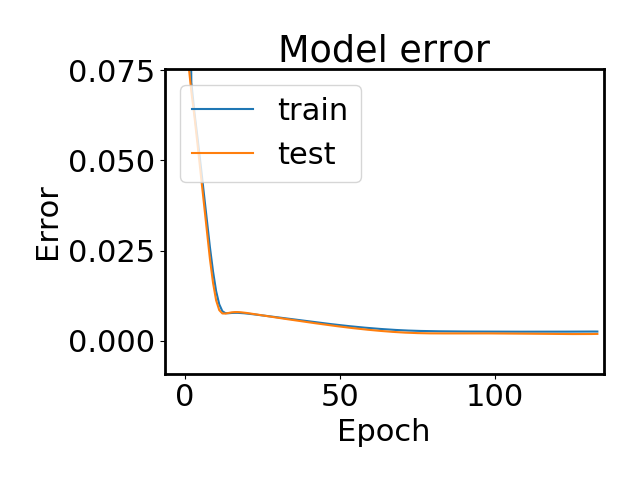
\includegraphics[width = \textwidth]{report/figures/analysis/lstm_gridsearch/best_lstm_error_zoomed.png}
                        \caption{Training history for the best LSTM configuration}
                        \label{fig:lstm_grid_error_best}
                    \end{minipage}
                    \begin{minipage}[b]{0.5\linewidth}
                        \centering
                        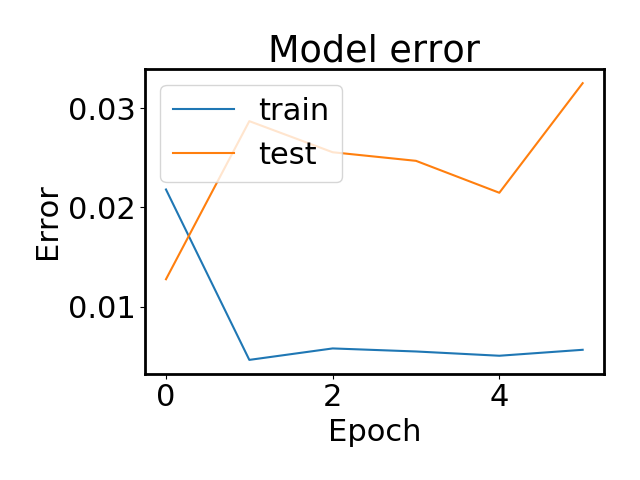
\includegraphics[width = \textwidth]{report/figures/analysis/lstm_gridsearch/worst_lstm_error_-1.png}
                        \caption{Training history for the worst LSTM configuration}
                        \label{fig:lstm_grid_error_worst}
                    \end{minipage}
                \end{figure}
        
    \section{Anomaly detection}
        Of the three methods used in the analysis, only one class SVM is a classifier. This means that only one class SVM will classify a sample as normal or abnormal. KDE and LSTM RNN gives an anomaly score, hence they will be referenced as anomaly scorers. This means that to identify a sample as an anomaly, one needs to find a threshold for the anomaly score. This is not covered in the thesis.  
        
    \subsection{Training case 1}
        \begin{figure}
            \centering
            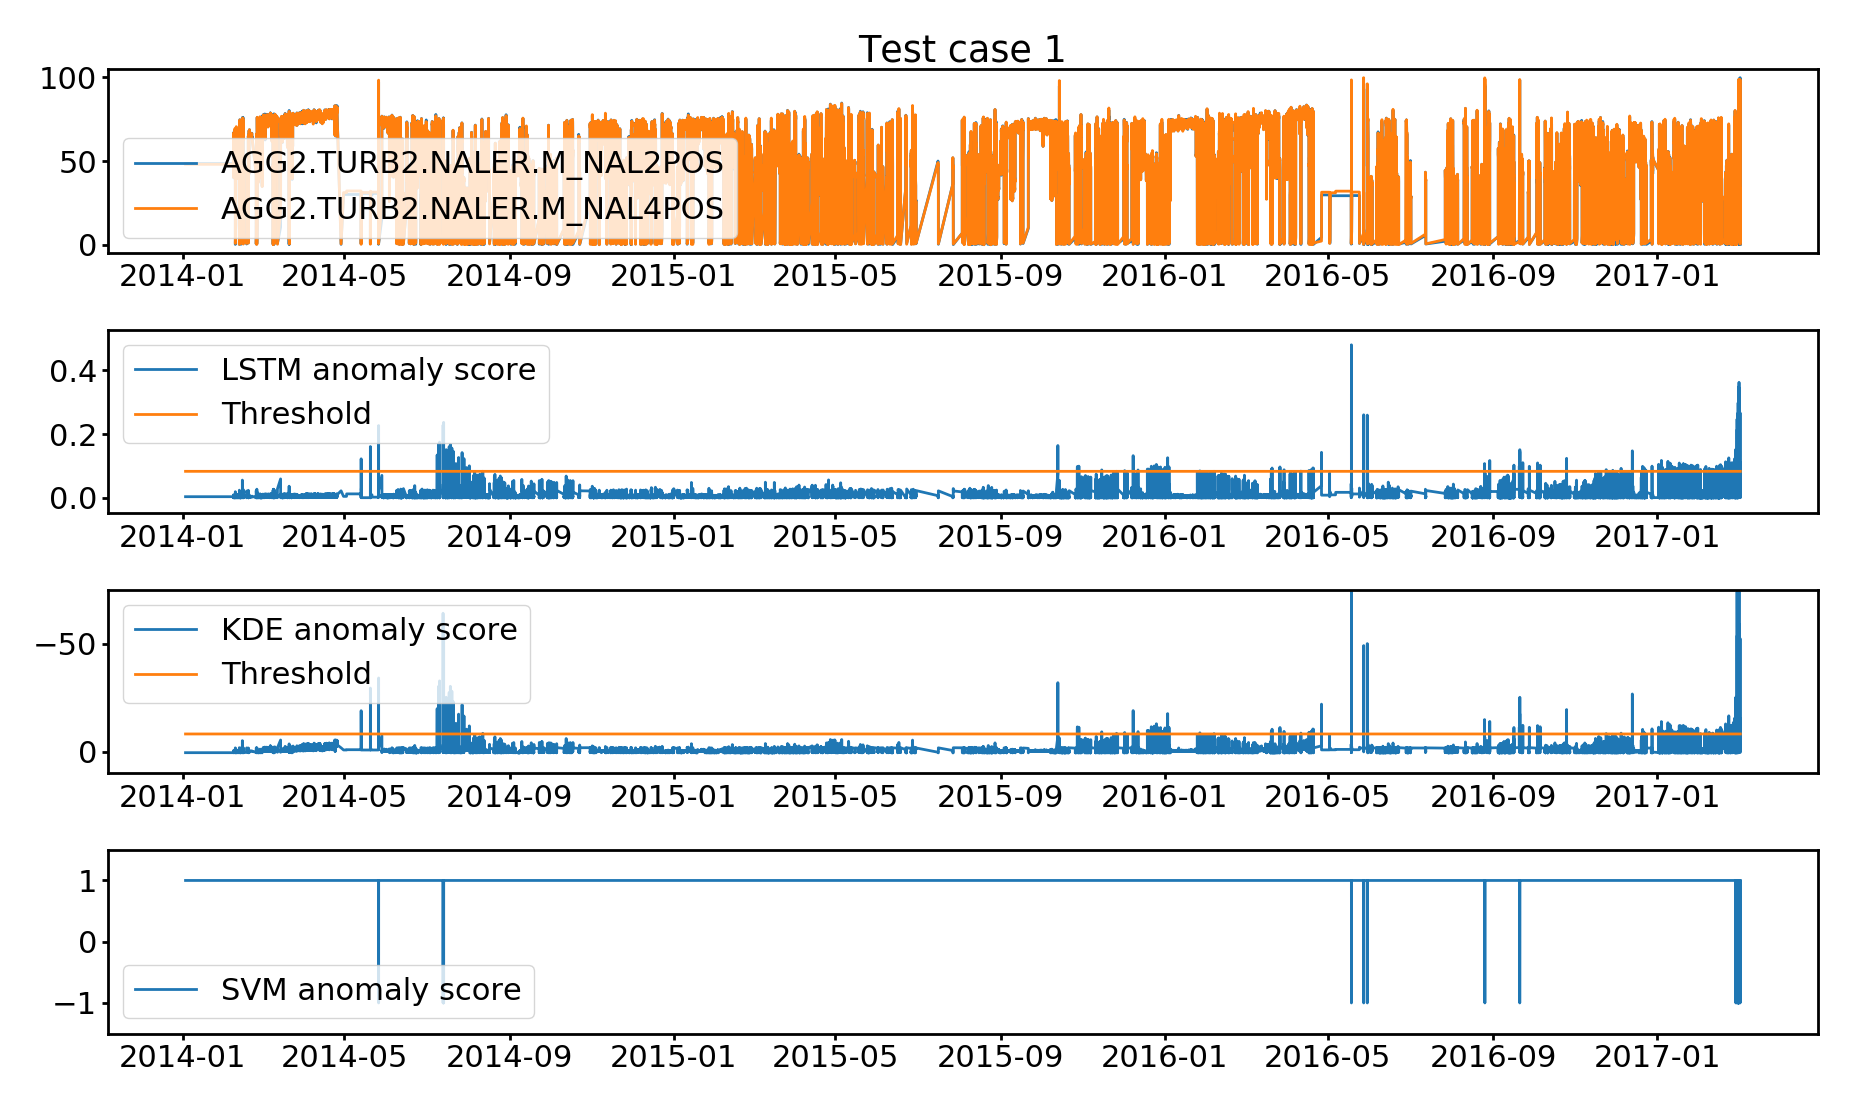
\includegraphics[width = \textwidth]{report/figures/analysis/plant1_training/production_data_anomaly.png}
            \caption{Anomaly score for the training set 1 on test case 1}
            \label{fig:anomaly_plant_1_train_production}
        \end{figure}
        Figure \ref{fig:anomaly_plant_1_train_production} shows the anomaly scores for the three different methods on case 1. The top window shows the opening of the two needles in case 1. As can be seen, it is hard to spot any deviation between the two needles from this plot. Window two from the top shows the anomaly scores for the LSTM scorer. The higher the score, the more abnormal the data is evaluated to be. Window three from the top shows the score for the KDE scorer. Here the more negative the score is, the more abnormal the data is. The bottom window shows the one class SVM classifier. A $1$ indicates that the data is classified as normal, and $-1$ as an anomaly. In the LSTM and KDE scorer windows, an orange line is plotted to indicate a constant anomaly threshold. The threshold is here set to a value that classifies $0.1\%$ of the data as anomalies. This is just to give an indication on how the data is distributed. Finding a reasonable value for the threshold would require expert knowledge about the operation of Pelton turbines, and having a constant value might be a to simple scheme. 
        
        For both the KDE and the LSTM anomaly scorers one can clearly see that the anomaly score of the data is gradually increasing from September 2016. Several samples after January 2017 are located above the proposed threshold line. The anomaly score for both scorers is more than doubled from the score seen during the lowest periods. This shows that one can clearly identify that the scorers are detecting patterns in the data not seen during training, in the period leading up to the incident. Interestingly, there are also several samples spread out over the entire sampling period that is given a high anomaly score. This can be because the training set does not cover all modes of operation, operational problems, or problems with data sampling. The power plant log did not report any operational issues except for the one seen in 2017, but from the authors experience from the industry, it is not uncommon that not all maintenance work is logged. The one class SVM classifier is not able to detect a trend building up towards the incident. As can be seen, it only evaluates a few anomalies in the period up until the reported incident. There are also signs of abnormalities earlier in the production data as seen for the anomaly scorers. Interestingly, one can see that the samples evaluated as anomalies for the one class SVM are all among the highest scoring samples for the two anomaly scorers. 
        
        Table \ref{tab:trainining_plant1_stats} shows how the scorers evaluate the validation data compared to the data from case 1. The plot for the anomaly scores on the validation and training sets can be found in appendix \ref{appendix:training_case1}, in addition, boundary plots for the SVM classifier, KDE scorer and learning history plots for the LSTM scorer can be found there. As can be seen, there is a large difference between the minimum values for the validation and case data for the KDE scorer, there is also a difference between the mean values. This shows that the case data takes on patterns not seen in the training data. The same trend is seen in the statistics for the LSTM scorer. In both cases, the most extreme observation between training and production is approximately 100 times larger.
        
        Figure \ref{fig:svm_1_outliers_stats_production} shows number and percentage of anomalies for the one class SVM classifier for the case 1 data. As can be seen, it only detects a small number of anomalies for the incidents seen in 2014 and 2016, but for the reported incident in 2017 one can see that the anomaly percentage is close to $50\%$. This gives an indication that separating what could be false positives from true positives could be solved by using a percentage threshold. 
        
        \begin{table}[]
            % \begin{minipage}[b]{0.48\linewidth}
            \centering
            \begin{tabular}{|c|c|c|c|c|}
                \hline
                            & KDE validation  & KDE case 1    & LSTM validation & LSTM case 2   \\ \hline
                min         & -2.671    & -275.66           & 1.659e-04 & 9.716e-05         \\ \hline
                max         & 0.491     & 0.491             & 3.032e-2  & 0.400             \\ \hline
                mean        & -0.296    & -0.728            & 3.318e-03 & 6.200e-3          \\ \hline
            \end{tabular}
            \caption{Table comparing the statistics for the KDE and LSTM anomaly detectors on the validation and case 1 data for training case 1}
            \label{tab:trainining_plant1_stats}
        \end{table}
        
        \begin{figure}
            \begin{minipage}[b]{0.49\linewidth}
                \centering
                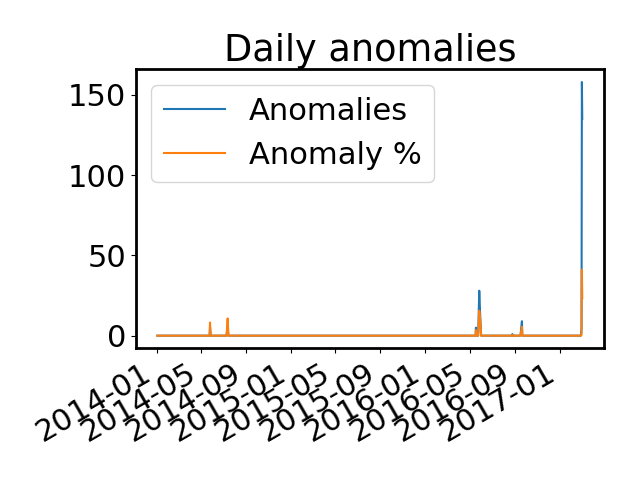
\includegraphics[width=\textwidth]{report/figures/analysis/plant1_training/daily_svm_outliers_production_small.png}
                \caption{Daily classified anomalies for the one class SVM classifier on production data}
                \label{fig:svm_1_outliers_stats_production}
            \end{minipage}
            \hfill\vline\hfill
            \begin{minipage}[b]{0.49\linewidth}
                \centering
                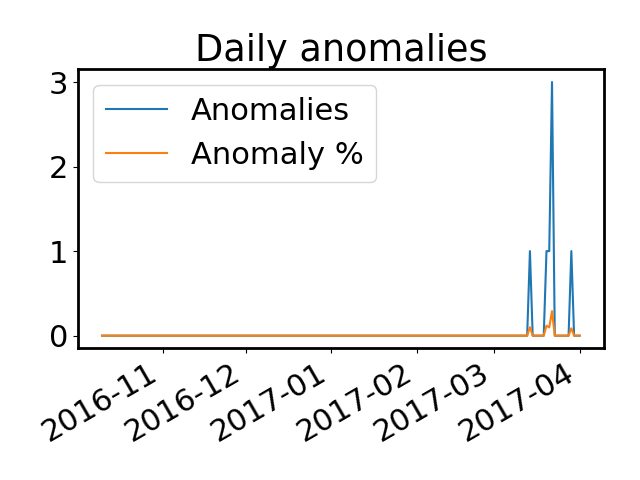
\includegraphics[width=\textwidth]{report/figures/analysis/plant1_training/daily_svm_outliers_artificial_small.png}
                \caption{Daily classified anomalies for the one class SVM classifier on artificial data}
                \label{fig:svm_1_outliers_stats_artificial}
            \end{minipage}
        \end{figure}
        
        Figure \ref{fig:anomaly_plant_1_train_artificial} shows the anomaly scores for the artificial data. Note that the artificial data and test case 1 is from different plants. There is no sample data from January 2017, but since dates are used as indexes, January is still seen in the plot. The data from 2016 is normal data from plant 2, and the artificial error is gradually increasing from February to April in 2017. As can be seen, both the LSTM and KDE scorers detect anomalies from mid-February. Towards march, the anomaly scores are significantly higher than for the normal data. The one class SVM classifier is not picking up the trend as fast as, but it clearly detects that something is wrong towards the end of the sample period. This can be verified by looking at \ref{fig:svm_1_outliers_stats_artificial}. \todo{Fix this plot? why is it only going to three samples?}     
        \begin{figure}
            \centering
            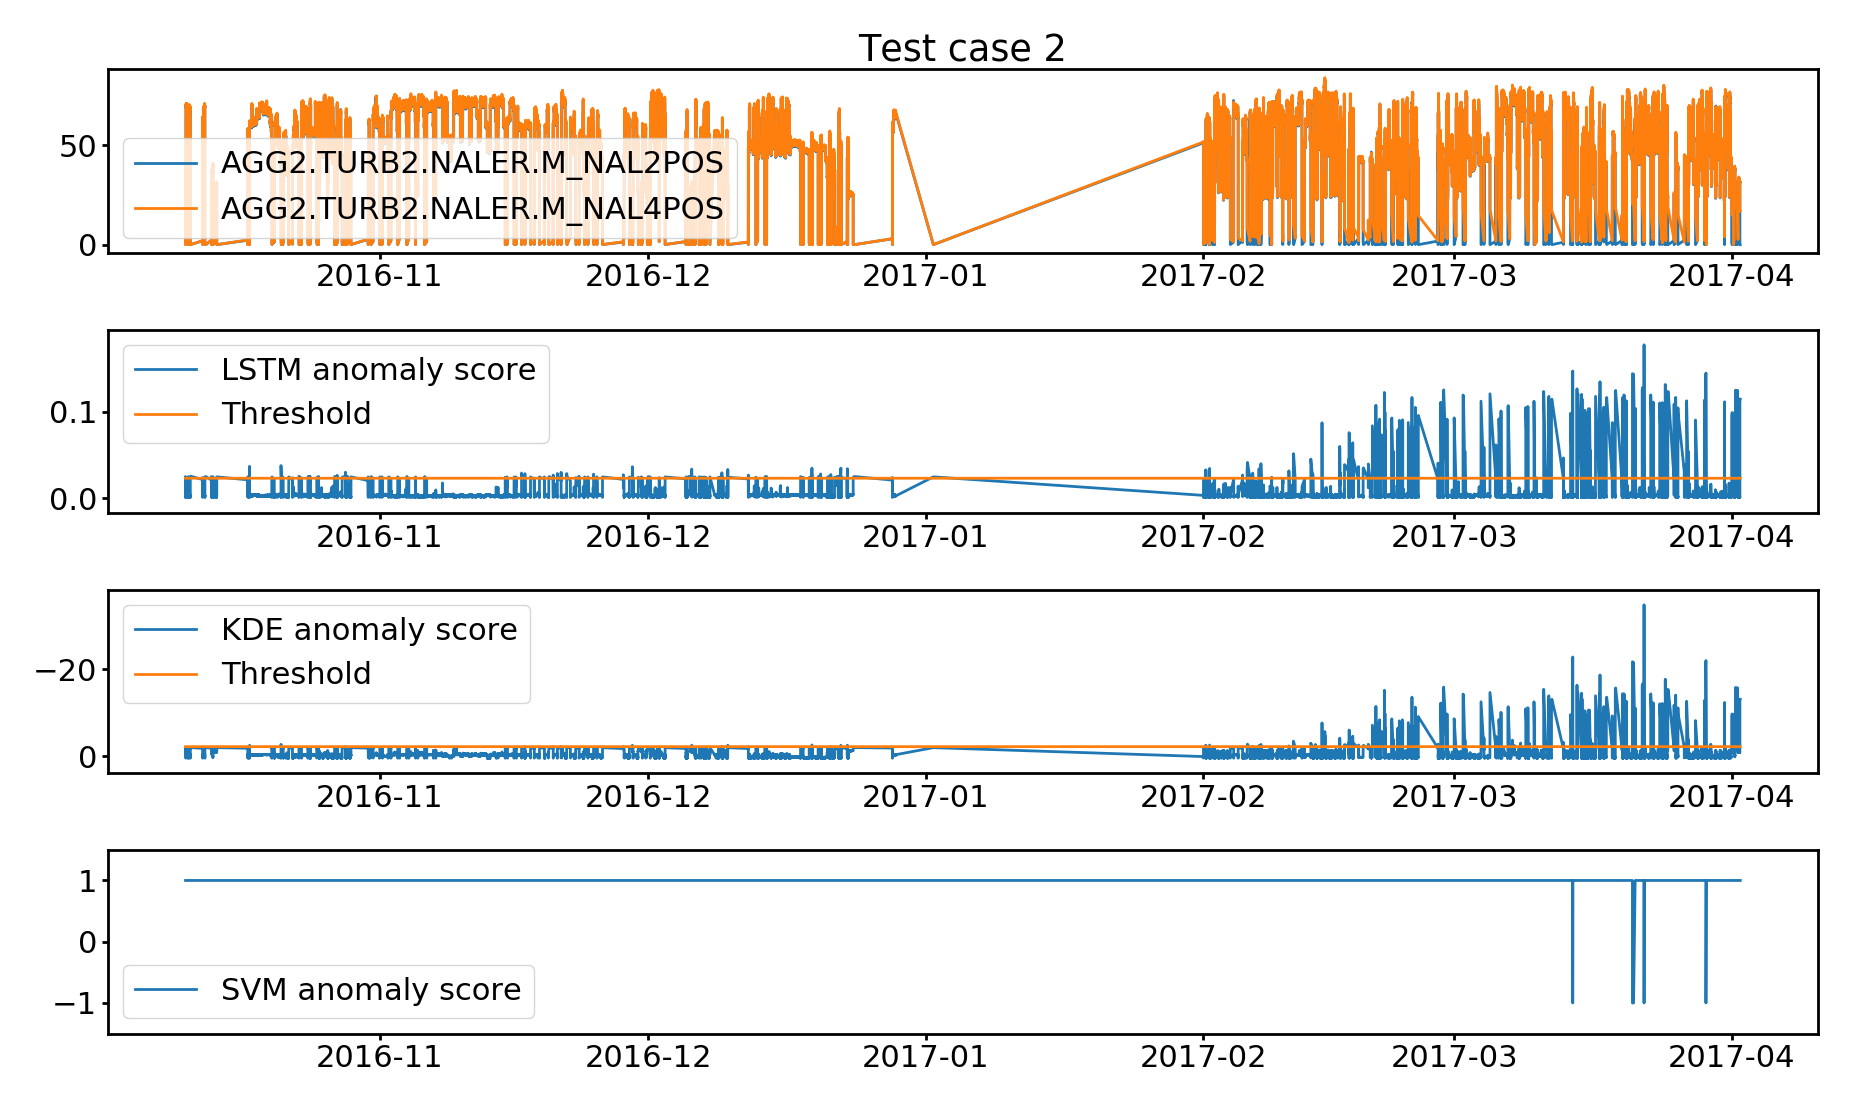
\includegraphics[width = \textwidth]{report/figures/analysis/plant1_training/artificial_data_anomaly.png}
            \caption{Anomaly score for training set 1 on test case 2}
            \label{fig:anomaly_plant_1_train_artificial}
        \end{figure}
    
    \subsection{Training case 2}
        \begin{figure}[h!]
            \centering
            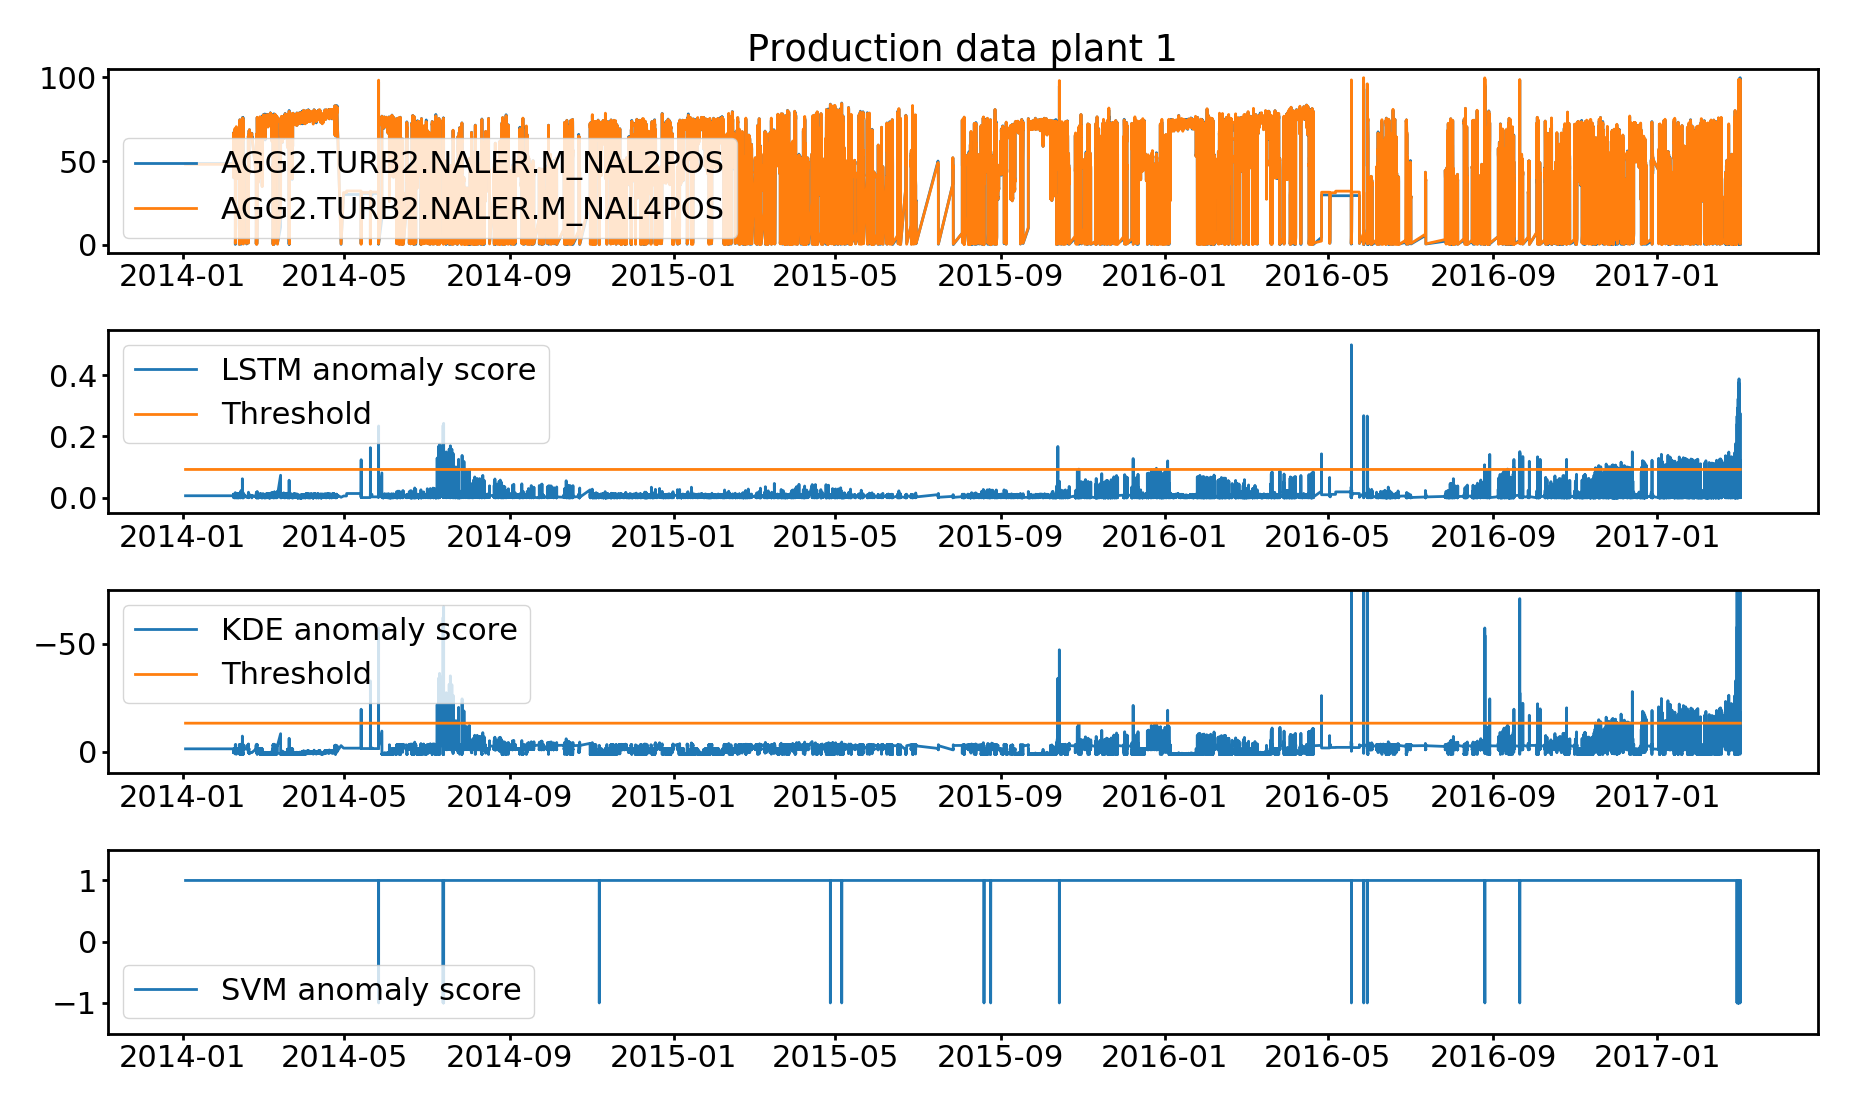
\includegraphics[width=\textwidth]{report/figures/analysis/plant2_train_short/production_data_anomaly.png}
            \caption{Anomaly score for training set 2 on test case 1}
            \label{fig:plant2_short_prod_anomaly_score}
        \end{figure}
        Figure \ref{fig:plant2_short_prod_anomaly_score} shows the anomaly scores for the production data in case 1, when trained on training case $2$. Training case 1 and 2 are as mentioned approximately of the same size. The figure shows a very similar pattern to training case $1$ for the two anomaly scorers. This could mean that both methods generalize well across plants, at least as long as the training sets are of similar size. 
        
        The biggest difference is seen in the one class SVM window, where there are some new samples being classified as anomalies in 2015. This could show that the one class SVM is more sensitive to the training data, as the data from 2015 seems to be the best data from this needle pair. However, looking at figure \ref{fig:svm_2_outliers_stats_production} it becomes clear that the number of new anomalies detected by training case $2$ in 2015 is small, and that setting a threshold as mentioned in the previous section could classify them as false positives.  
        
        Table \ref{tab:trainining_plant2_short_stats} shows the anomaly statistics for training case $2$. It is clear that both scorers have a higher minimum and maximum values than what was seen for case $1$. This means that the data from the reported incident is given a higher anomaly score for training case 2 than for case 1. This is interesting since training case 2 is sampled from another plant. However, the mean values for both scorers are also changed, which could indicate that score is simply biased. 
        \begin{table}[]
            \centering
            \begin{tabular}{|c|c|c|c|c|}
                \hline
                            & KDE validation  & KDE case 1     & LSTM validation     & LSTM case 1   \\ \hline
                min         & -4.566        & -296.370           & 2.336e-05            & 2.336e-05         \\ \hline
                max         & 1.291         & 1.2905             & 4.047e-2             & 0.498             \\ \hline
                mean        & --0.518       & -1.493             & 4.976e-04            & 8.116e-3          \\ \hline
            \end{tabular}
            \caption{Table comparing the statistics for the KDE and LSTM anomaly detectors on the validation and production data}
            \label{tab:trainining_plant2_short_stats}
        \end{table}
        \begin{figure}[h!]
            \begin{minipage}[b]{0.49\linewidth}
                \centering
                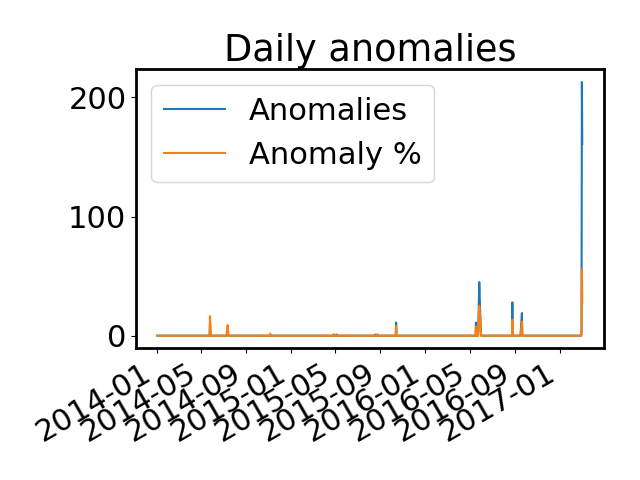
\includegraphics[width=\textwidth]{report/figures/analysis/plant2_train_short/daily_svm_outliers_production_small.png}
                \caption{Anomaly statistics for one class SVM on production data}
                \label{fig:svm_2_outliers_stats_production}
            \end{minipage}
            \hfill\vline\hfill
            \begin{minipage}[b]{0.49\linewidth}
                \centering
                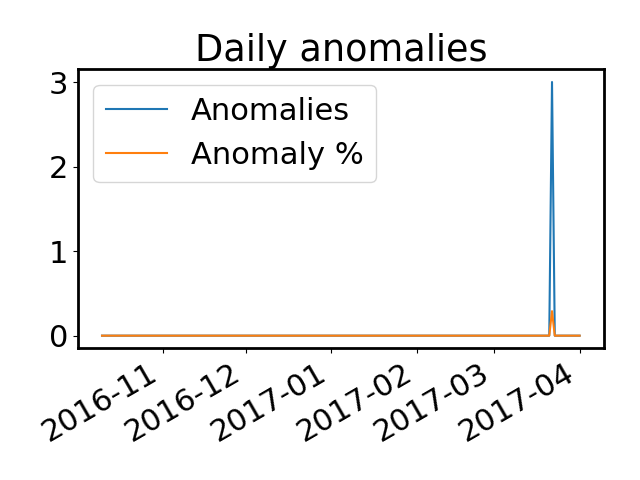
\includegraphics[width=\textwidth]{report/figures/analysis/plant2_train_short/daily_svm_outliers_artificial_small.png}
                \caption{Anomaly statistics for one class SVM on artificial data}
                \label{fig:svm_2_outliers_stats_artificial}
            \end{minipage}
        \end{figure}
        
        \begin{figure}[h!]
            \centering
            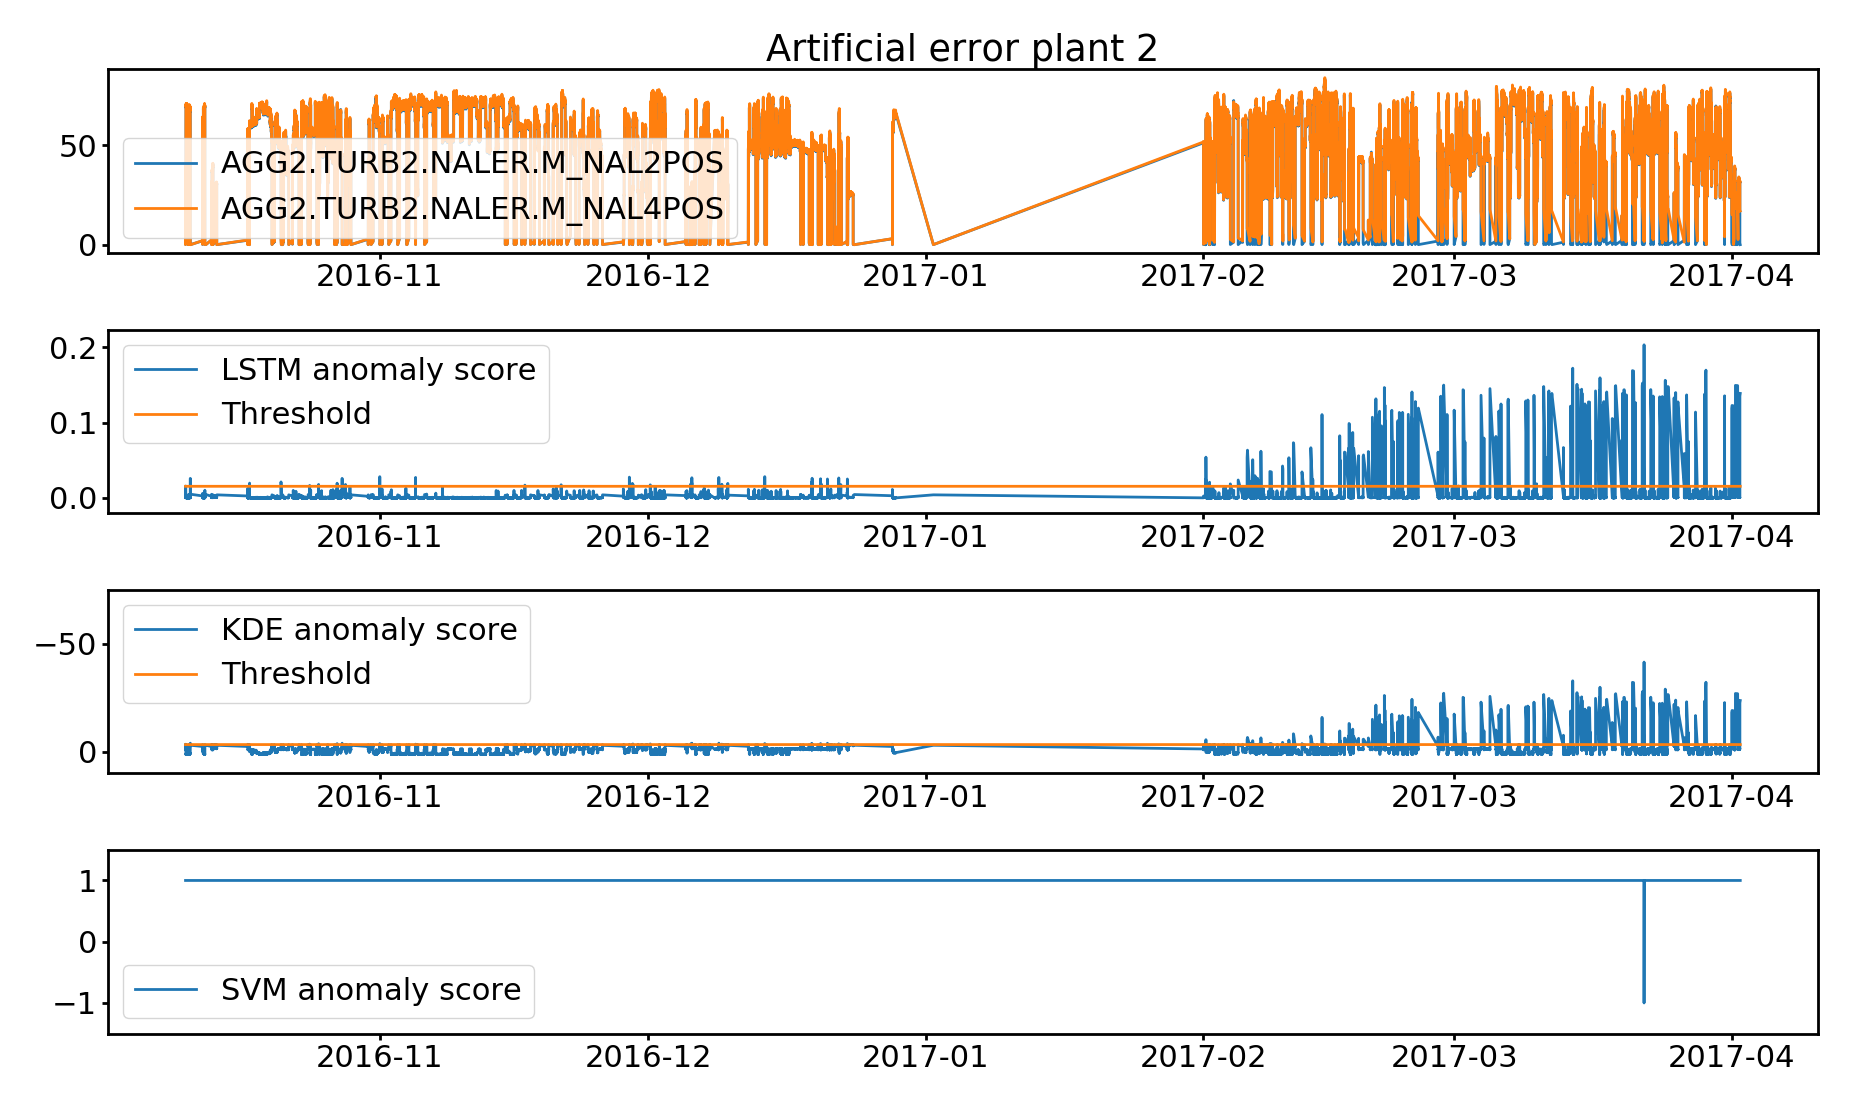
\includegraphics[width=\textwidth]{report/figures/analysis/plant2_train_short/artificial_data_anomaly.png}
            \caption{Anomaly score for training set 2 on test case 2}
            \label{fig:plan2_short_arti_anomaly_score}
        \end{figure}
        Figure \ref{fig:plan2_short_arti_anomaly_score} shows the anomaly scores for the artificial data in case 2. As with case 1, both scorers behave very similar to what was seen for training set 1. Looking at the LSTM anomaly score in window two, one can verify that the anomaly score increases immediately after the error is applied. It is able to detect only small deviation from the normal operating pattern. The  KDE scorer also seems to pick up the artificial error faster than for training set 1. As the artificial error is added to process data from the same needle pair as the training data for case 2, it is sensible that it is possible to detect the anomalies earlier than for training case 1.   
        
        The one class SVM detector is, however, having problems detecting the anomalies, and only detects the sample that the two other detectors identify as the most anomalous. Note that the training case here is based on normal data from plant 2. One possible explanation to this is that the parameters found in the hyperparameterization for the one class SVM do not generalize very well to new data, as the hyperparameterization was performed on data from plant 1.
        
        
    
    \subsection{Training case 3}
        \begin{figure}[h!]
            \centering
            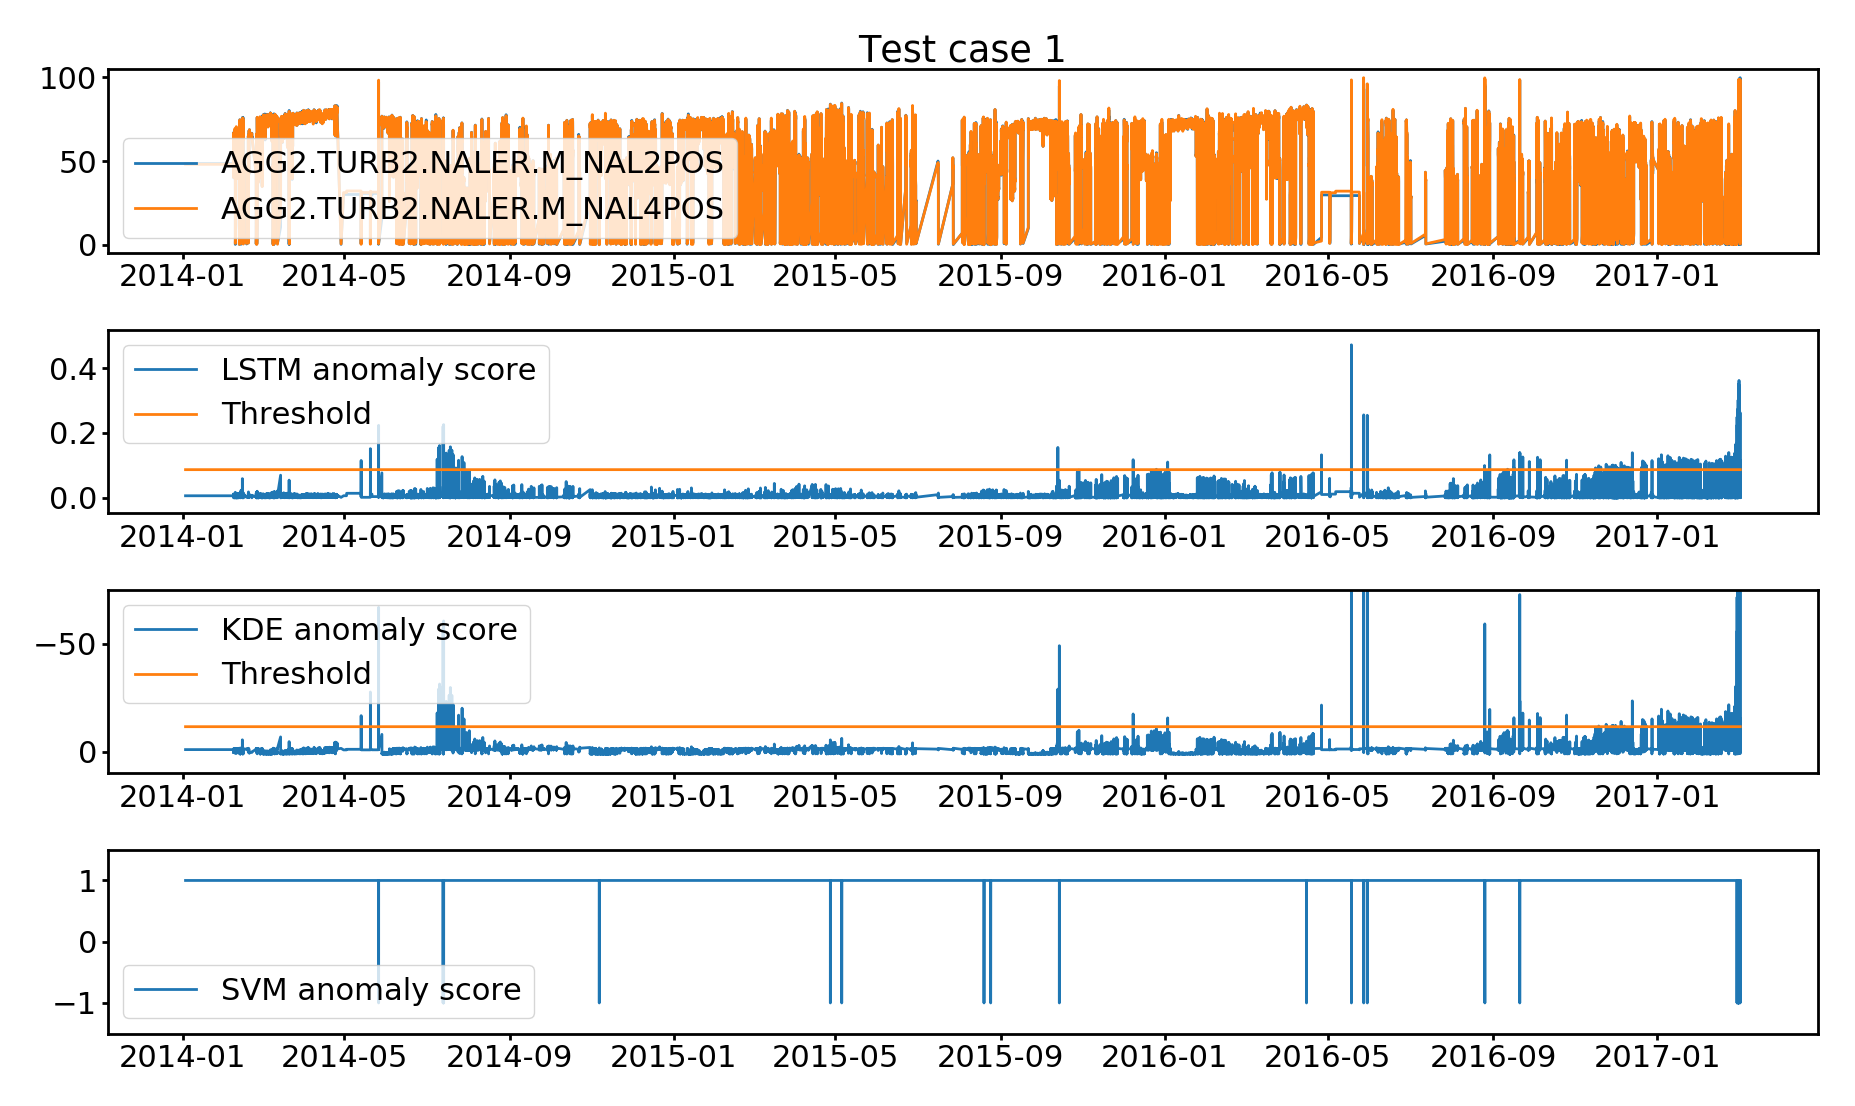
\includegraphics[width=\textwidth]{report/figures/analysis/plant2_train_long/production_data_anomaly.png}
            \caption{Anomaly score for training set 3 on test case 1}
            \label{fig:plant2_lomg_prod_anomaly_score}
        \end{figure}
        Figure \ref{fig:plant2_lomg_prod_anomaly_score} shows the anomaly scores and classifications for the production data in case 1 when trained on training set $3$. It is ten times larger than training set $1$ and $2$. As with set $2$, the scorers evaluate anomalies very similar to what was seen for training set $1$. Both scorers detect a rising trend of abnormal data towards the reported incident in March 2017. The anomaly scores for the data from the day of the incident is very high for both scorers, as was seen in the two previous cases as well. The one class SVM classifier is classifying the production data in case 1 very similar to training set 2, as is verified by figure \ref{fig:svm_3_outliers_stats_production}. Adding more data from plant 2 did not fix the issue with what appears to be false positives in the data sampled in 2015. 
        
        \begin{figure}[h!]
            \begin{minipage}[b]{0.49\linewidth}
                \centering
                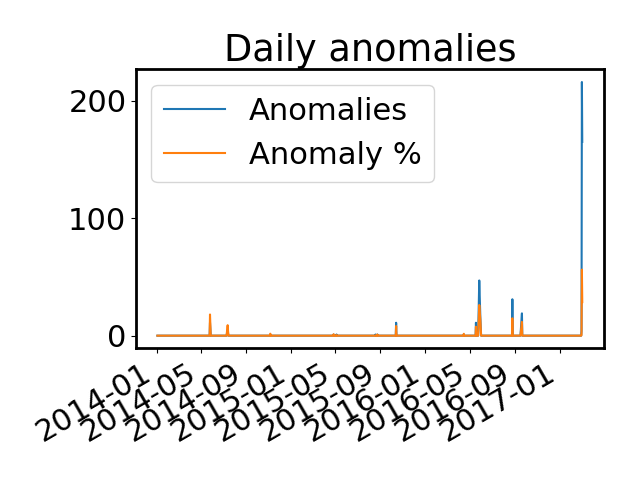
\includegraphics[width=\textwidth]{report/figures/analysis/plant2_train_long/daily_svm_outliers_production_small.png}
                \caption{Anomaly statistics for one class SVM on production data}
                \label{fig:svm_3_outliers_stats_production}
            \end{minipage}
            \hfill\vline\hfill
            \begin{minipage}[b]{0.49\linewidth}
                \centering
                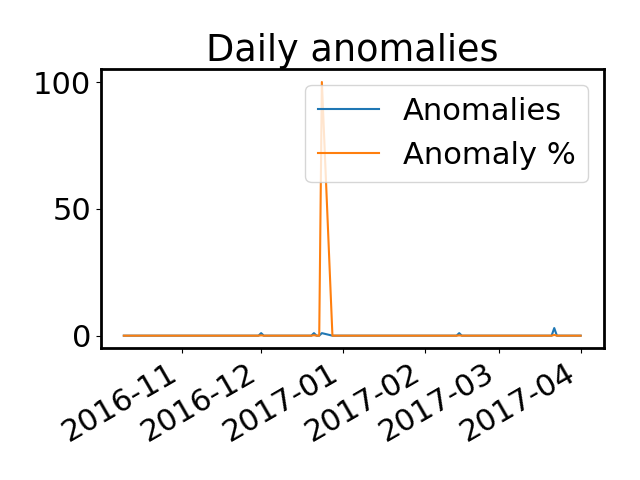
\includegraphics[width=\textwidth]{report/figures/analysis/plant2_train_long/daily_svm_outliers_artificial_small.png}
                \caption{Anomaly statistics for one class SVM on artificial data}
                \label{fig:svm_3_outliers_stats_artificial}
            \end{minipage}
        \end{figure}
        
        Table \ref{tab:trainining_plant2_long_stats} show the statistics for the LSTM and KDE detectors, the statistics are similar to what was seen in the previous training sets. Early stopping stopped the LSTM scorer after only 20 epochs, where the two previous sets ran for 134. When running the LSTM for 134 epochs, the performance of the LSTM scorer was much worse than for the previous training sets. This could indicate that the training set from case 2 holds the same information as case 3, but as case 3 has more samples, the algorithm does not need to iterate over the entire set as many times. Early stopping is used to avoid overfitting on the training data, and the poor performance when running for 134 epochs on set 3, is most likely due to overfitting. The fact that the two other methods appear to evaluate test case 1 similar for both training sets, further strengthens this. If the added data has a different distribution than the one in training set 2, this would have been caught by KDE and one class SVM.     
        \begin{table}[]
            \centering
            \begin{tabular}{|c|c|c|c|c|}
                \hline
                            & KDE validation  & KDE case 1     & LSTM validation & LSTM case 1   \\ \hline
                min         & -2.755    & -277.804              & 2.559e-05         & 2.796e-05         \\ \hline
                max         & 0.999     & 0.9995                & 3.597e-2          & 0.471             \\ \hline
                mean        & -0.366   & -1.167                 & 6.709e-04         & 7.651e-03          \\ \hline
            \end{tabular}
            \caption{Table comparing the statistics for the KDE and LSTM anomaly detectors on the validation and production data}
            \label{tab:trainining_plant2_long_stats}
        \end{table}




        % Figure \ref{fig:plan2_short_arti_anomaly_score} shows the anomaly scores for the artificial data. As with the production data from plant 1 both the KDE and LSTM detectors behave very similar to what was seen for training case 1. Looking at the LSTM anomaly score in window two, one can verify that the detector is able to track the artificial error from the date it is applied whereas for training case 1 it took a long time before the anomaly score indicated something abnormal. The one class SVM detector is, however, having problems detecting the anomalies, and only detects the sample that the two other detectors identify as the most abnormal. Note that the training case here is based on normal data from plant 2. It seems like the parameters found in the hyperparameterization of the one class SVM does not generalize very well to new data.
        \begin{figure}[h!]
            \centering
            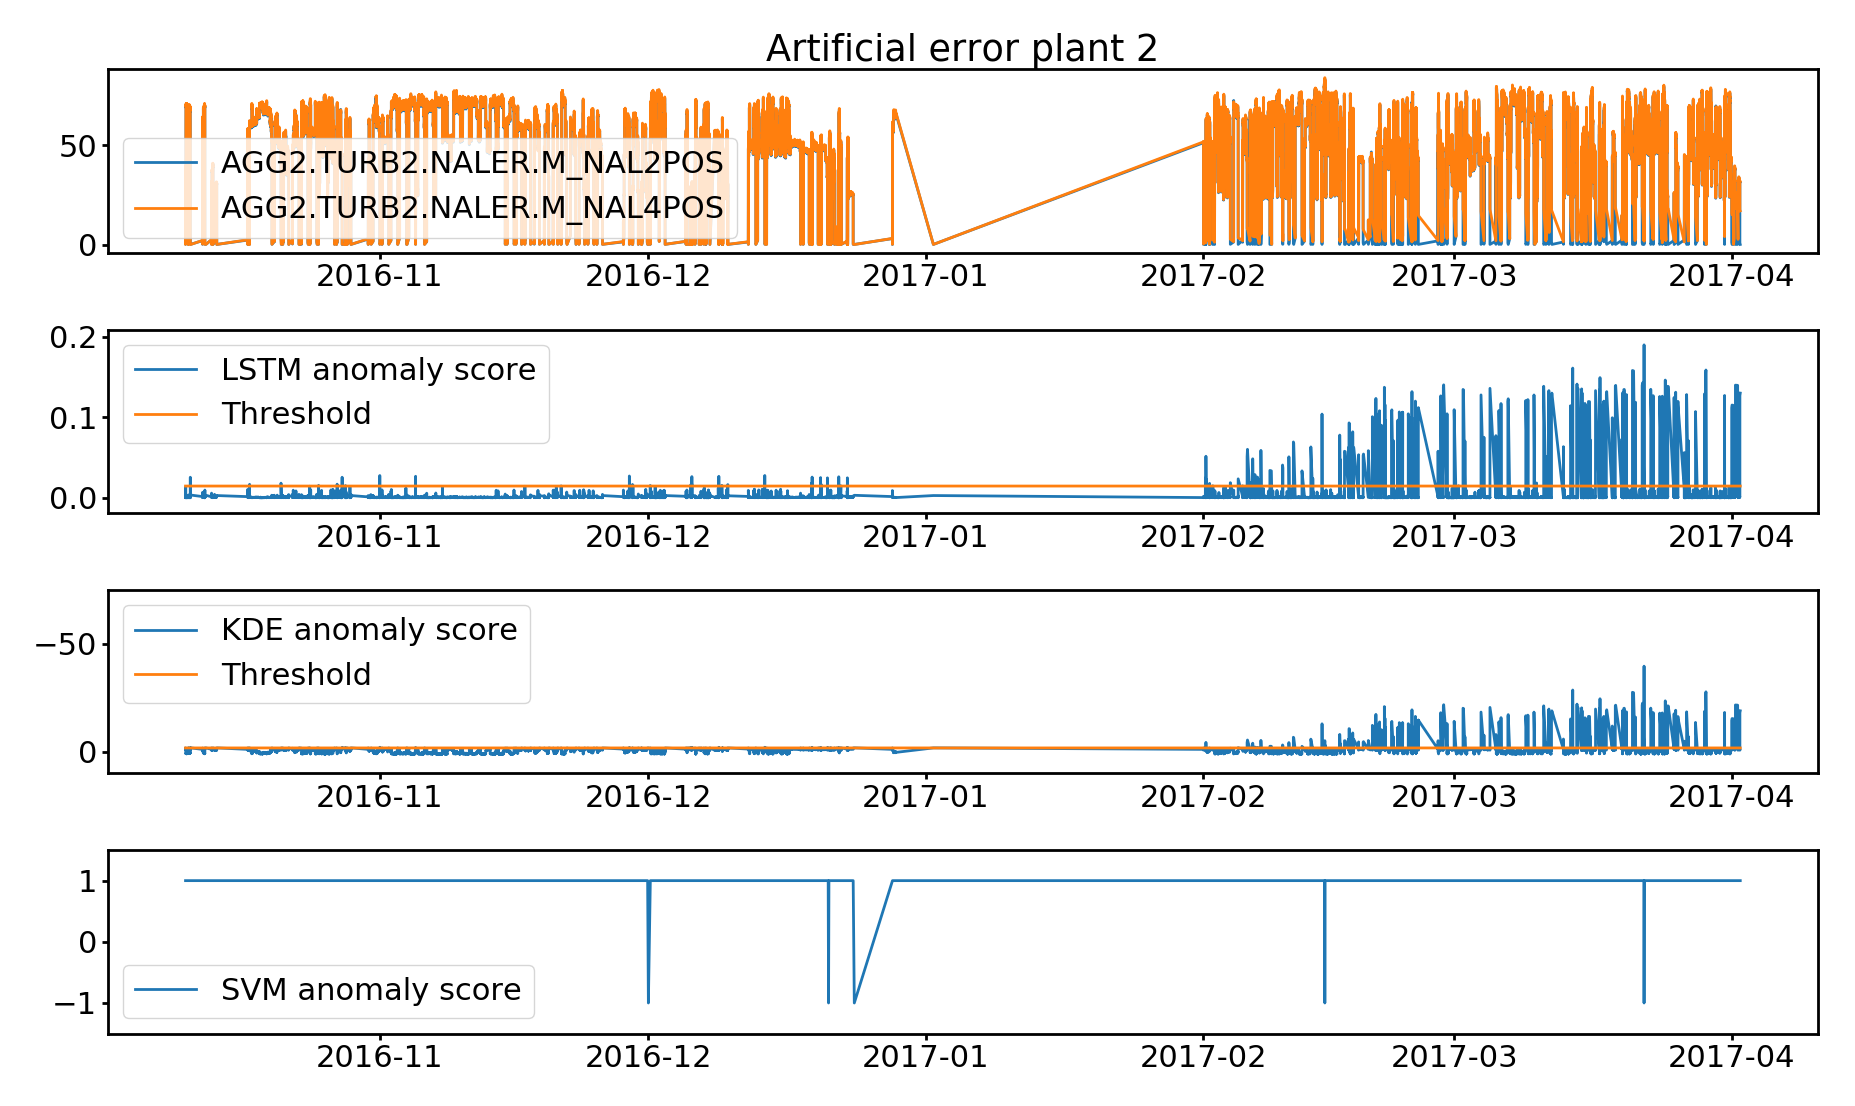
\includegraphics[width=\textwidth]{report/figures/analysis/plant2_train_long/artificial_data_anomaly.png}
            \caption{Anomaly score for training set 3 on test case 2}
            \label{fig:plan3_long_arti_anomaly_score}
        \end{figure}
        Figure \ref{fig:plan3_long_arti_anomaly_score} shows the anomaly scores for the artificial error data in case 2. Here as for the production data, one can verify that the scorers behave more or less equal to what was seen in training case $2$. The one class SVM classifier is showing a new pattern, by detecting anomalies in the normal test data, and is only able to classify data from one day during the artificial error as anomalous. This further strengthens the assumption that the one class SVM algorithm is sensitive to the combination of parameterization and training data. 
    
    
    
    \subsection{Comparing the three different training cases on production data}
        \begin{figure}[h!]
            \centering
            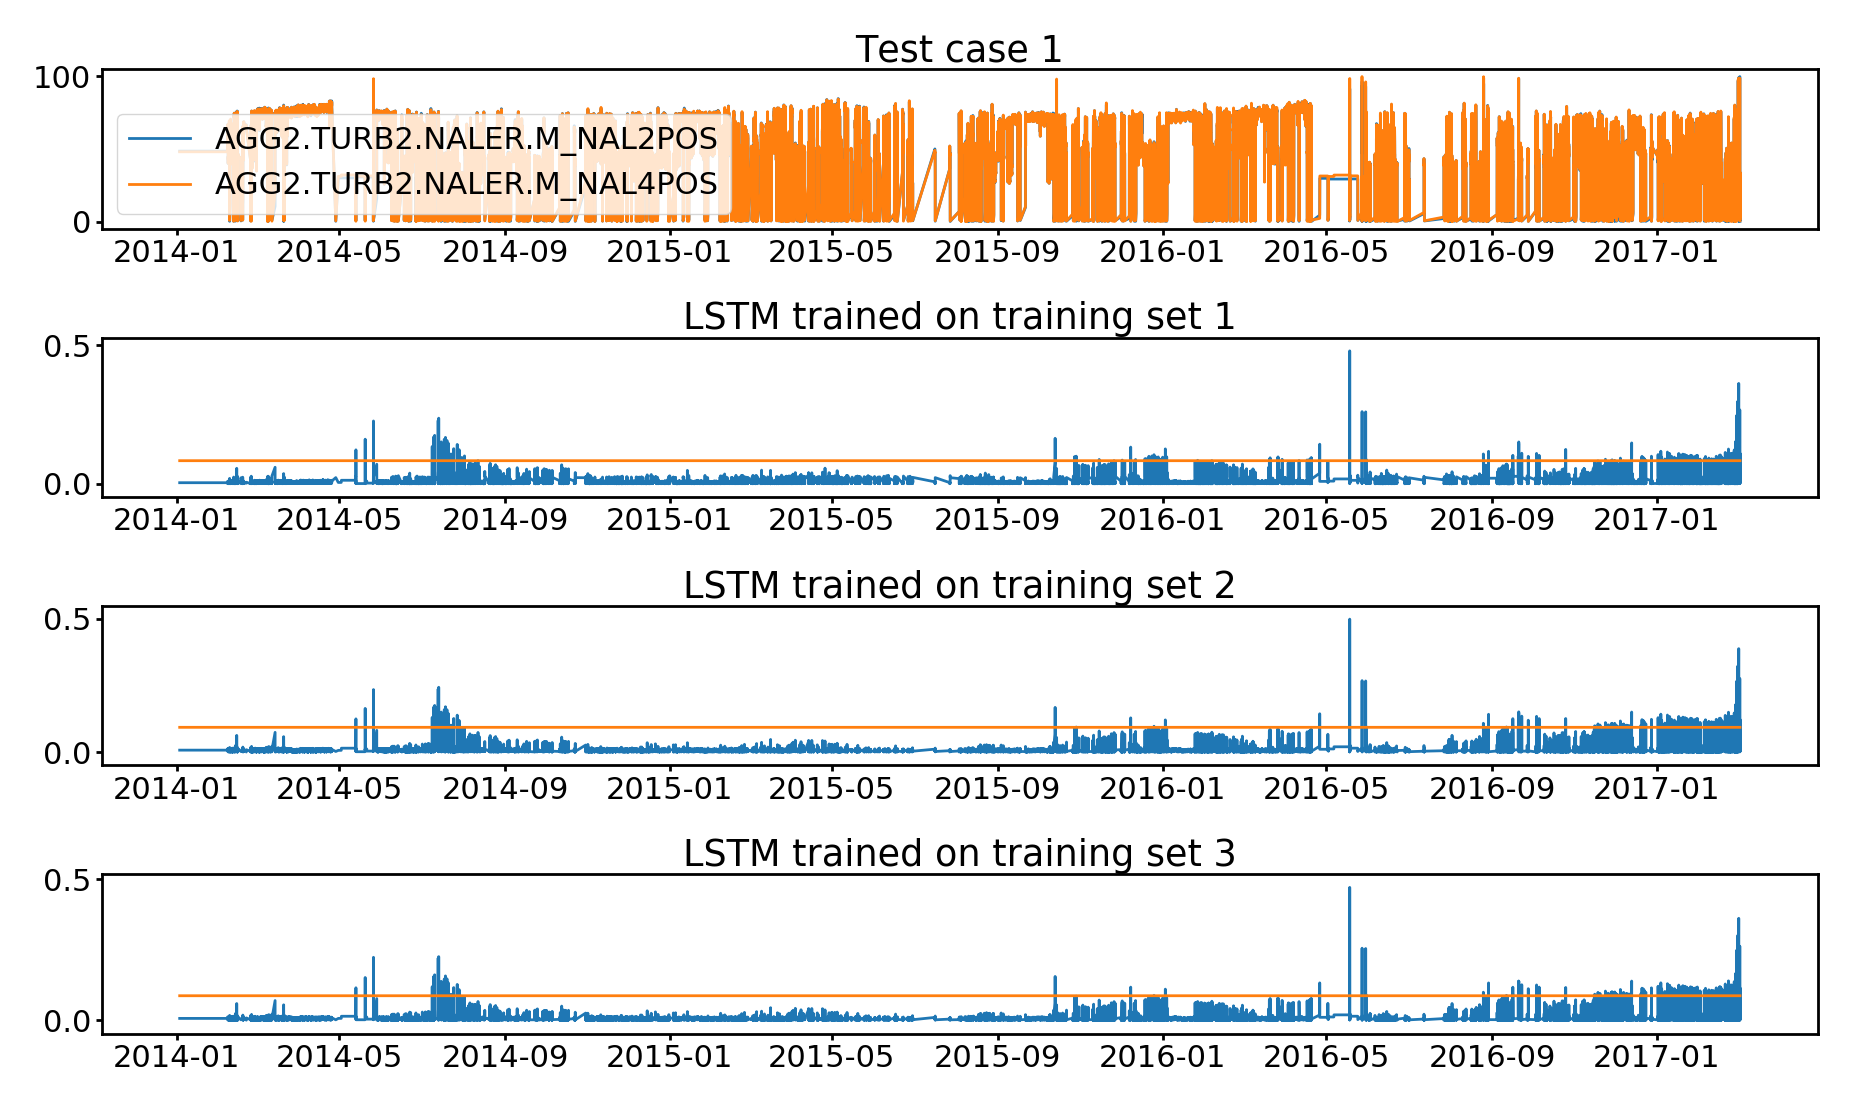
\includegraphics[width=\textwidth]{report/figures/analysis/training_cases/lstm_training_cases.png}
            \caption{All three LSTM training cases}
            \label{fig:lstm_training_cases}
        \end{figure}
        To simplify comparing the performance of the different methods new plots are created that shows how the different methods evaluate the production data in case 1, for all three training cases. Figure \ref{fig:lstm_training_cases} show case 1 evaluated by the three LSTM scorers. It is clear that all the scorers perform very similar. This shows that the method works well for both large and smaller training sets. All scores indicates a growing anomaly trend towards the incident in 2017, but the scorers for training set 2 and 3 show an increasing anomaly trend earlier than the scorer for set 1. A theory for why this is happening is that the training data used in set 1 is sampled right after maintenance, while the training sets from plant 2 are sampled after years of operation. This means that minor deviations between the needles that could be normal after some time of use, is seen as anomalous for the scorer trained on set 1 while this is seen as normal when set 2 and 3 are used for training. However, deploying any of the three scorers at the plant, could have warned about an increase in anomalous observations, that could have identified the anomalous trend before it is becoming too extreme. 
        
        \begin{figure}[h!]
            \centering
            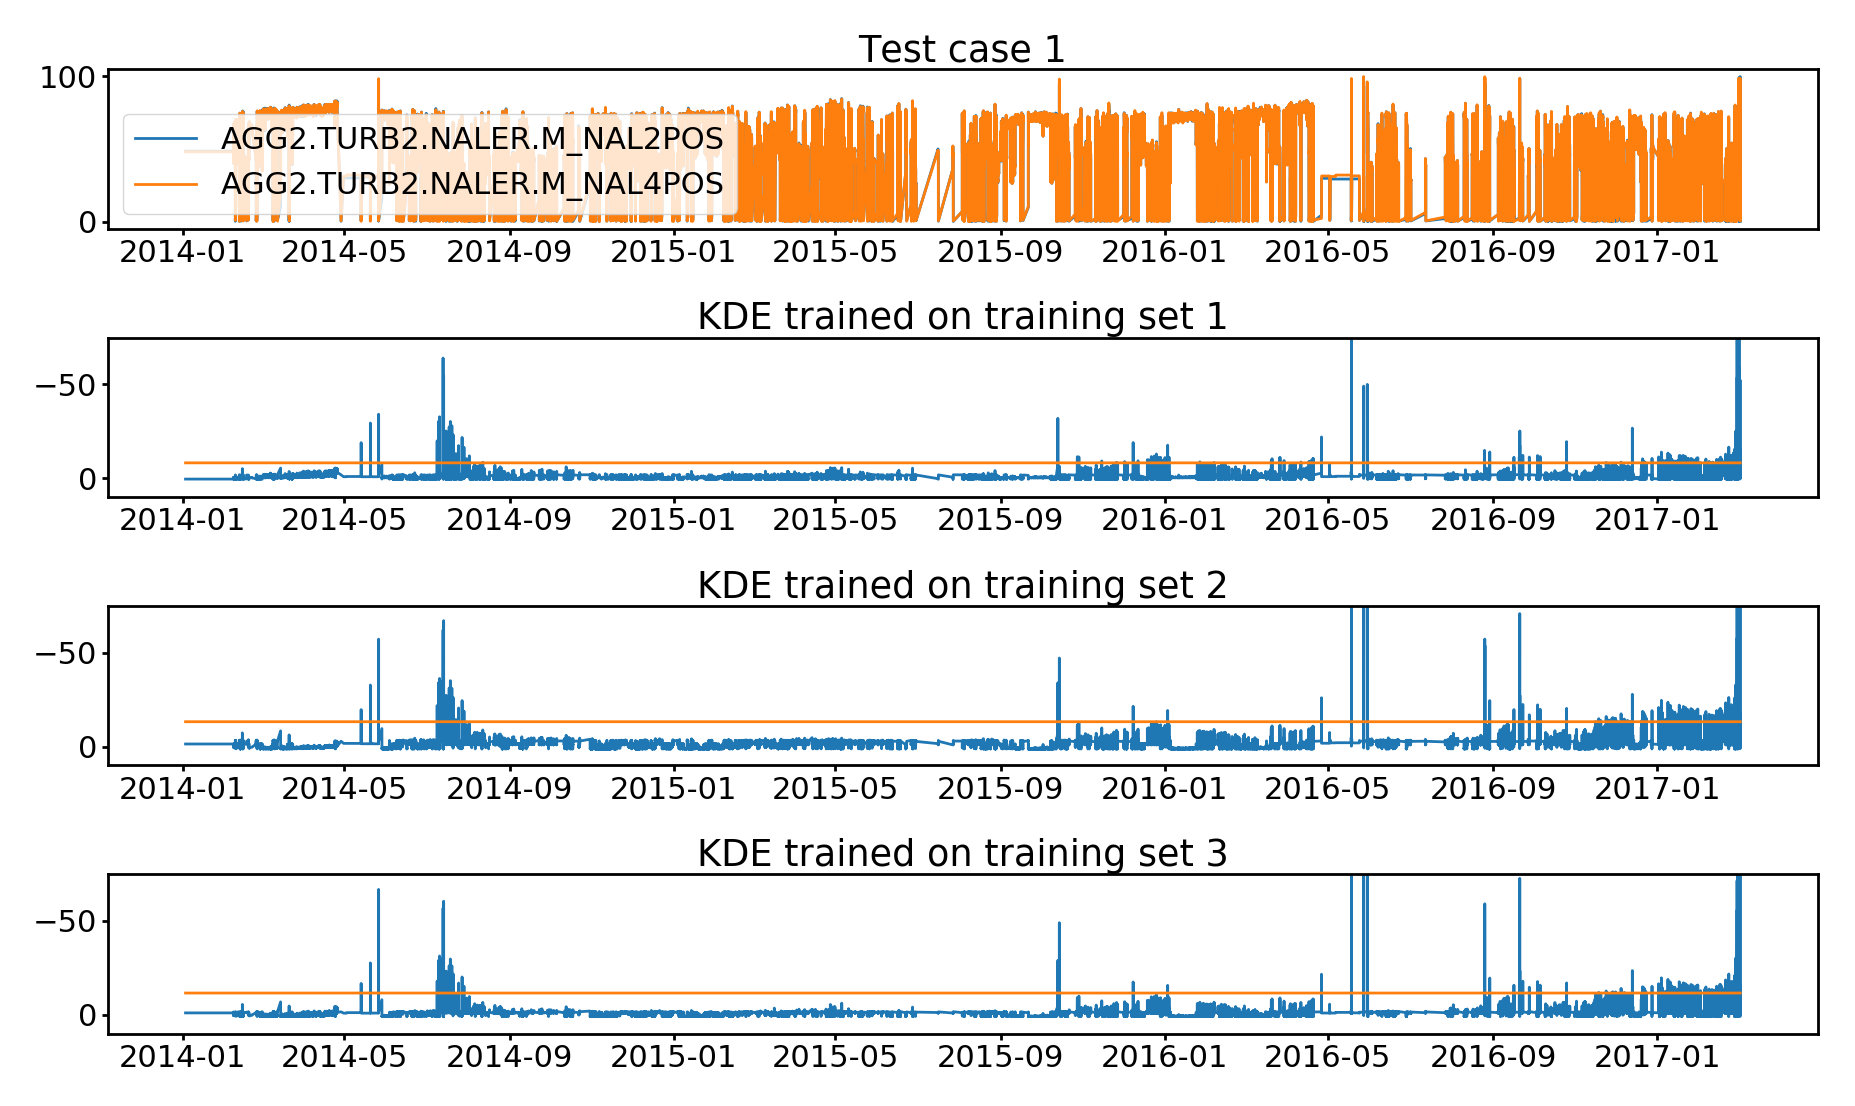
\includegraphics[width=\textwidth]{report/figures/analysis/training_cases/kde_training_cases.png}
            \caption{All three KDE training cases}
            \label{fig:kde_training_cases}
        \end{figure}
        Figure \ref{fig:kde_training_cases} shows how the different KDE scorers compare. All three scorers evaluate the test data very similar. The scorer from training set 2 is gives the highest anomaly scores for the data leading up to the incident. As with the LSTM scorers, set 2 and set 3 appears perform slightly better than set 1. All three scorers are able to detect the growing number of abnormal data seen towards March 2017. Notice that the score is limited to -75 to enable the reader to see the smaller trends, as the extreme values go below -250, making interpreting the plot very hard.
        
        \begin{figure}[h!]
            \centering
            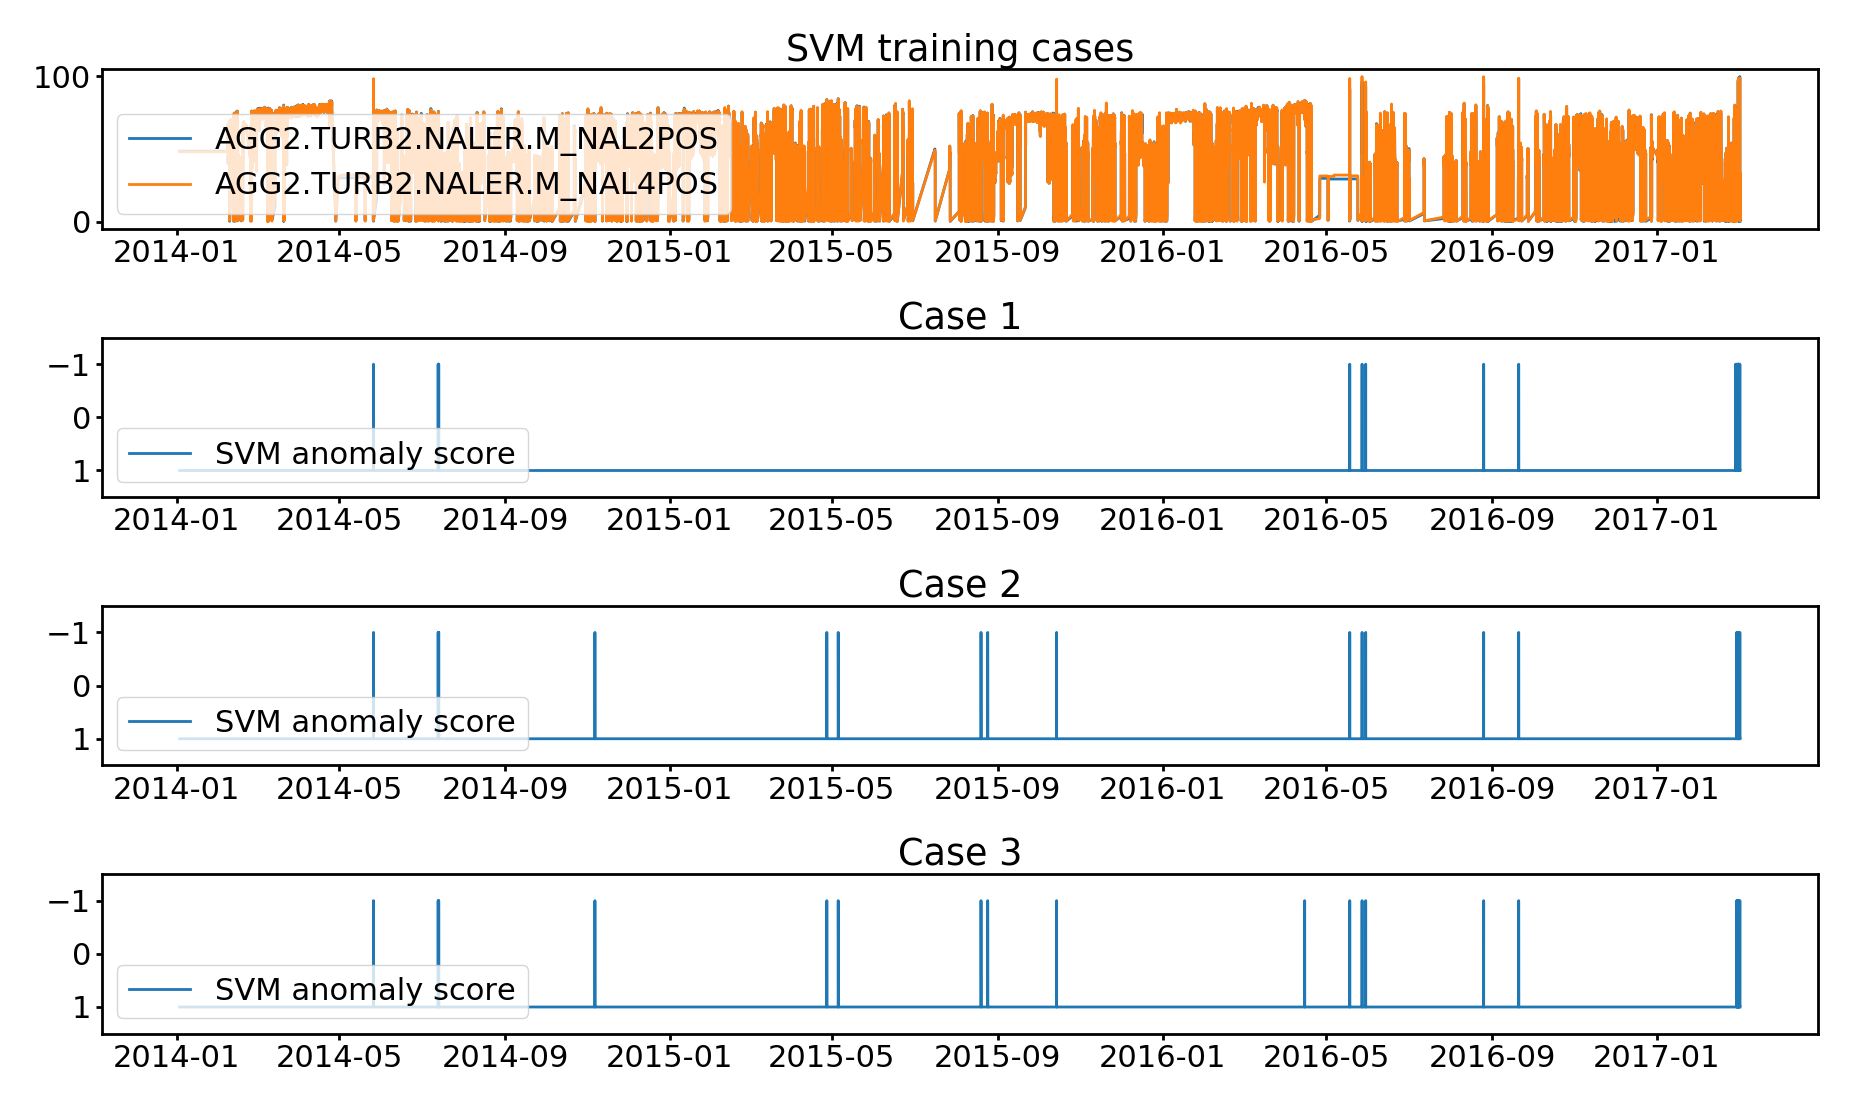
\includegraphics[width=\textwidth]{report/figures/analysis/training_cases/svm_training_cases.png}
            \caption{All three SVM training cases}
            \label{fig:svm_training_cases}
        \end{figure}
        Finally, figure \ref{fig:svm_training_cases} show the three different one class SVM classifiers. As with the two previous methods, there is little difference between set 2 and 3. This is the only method that appears to perform best when trained on data from plant 1. However, there is very little difference in the classifications, and when using the percentage of daily anomalies, one can easily separate the data from the incident with the other. This method is harder to spot trends with, and with the current parameterization, it is hard to find a way this method can be used as an early warning system for the incident seen in March 2017. This makes sense, as this method gives a predicts all data as either normal or anomalous, and hence include an extra step compared to KDE and LSTM which gives a score that the user need to interpret. Hence using this method would require less of the user, but more tuning and testing to ensure correct behaviour. 
        
    
    
    
    
    
    
    
    
    
    
    
    
    
    
    
    
    
    
    
    
    
    
    
    
    %     \begin{figure}
    %         \centering
    %         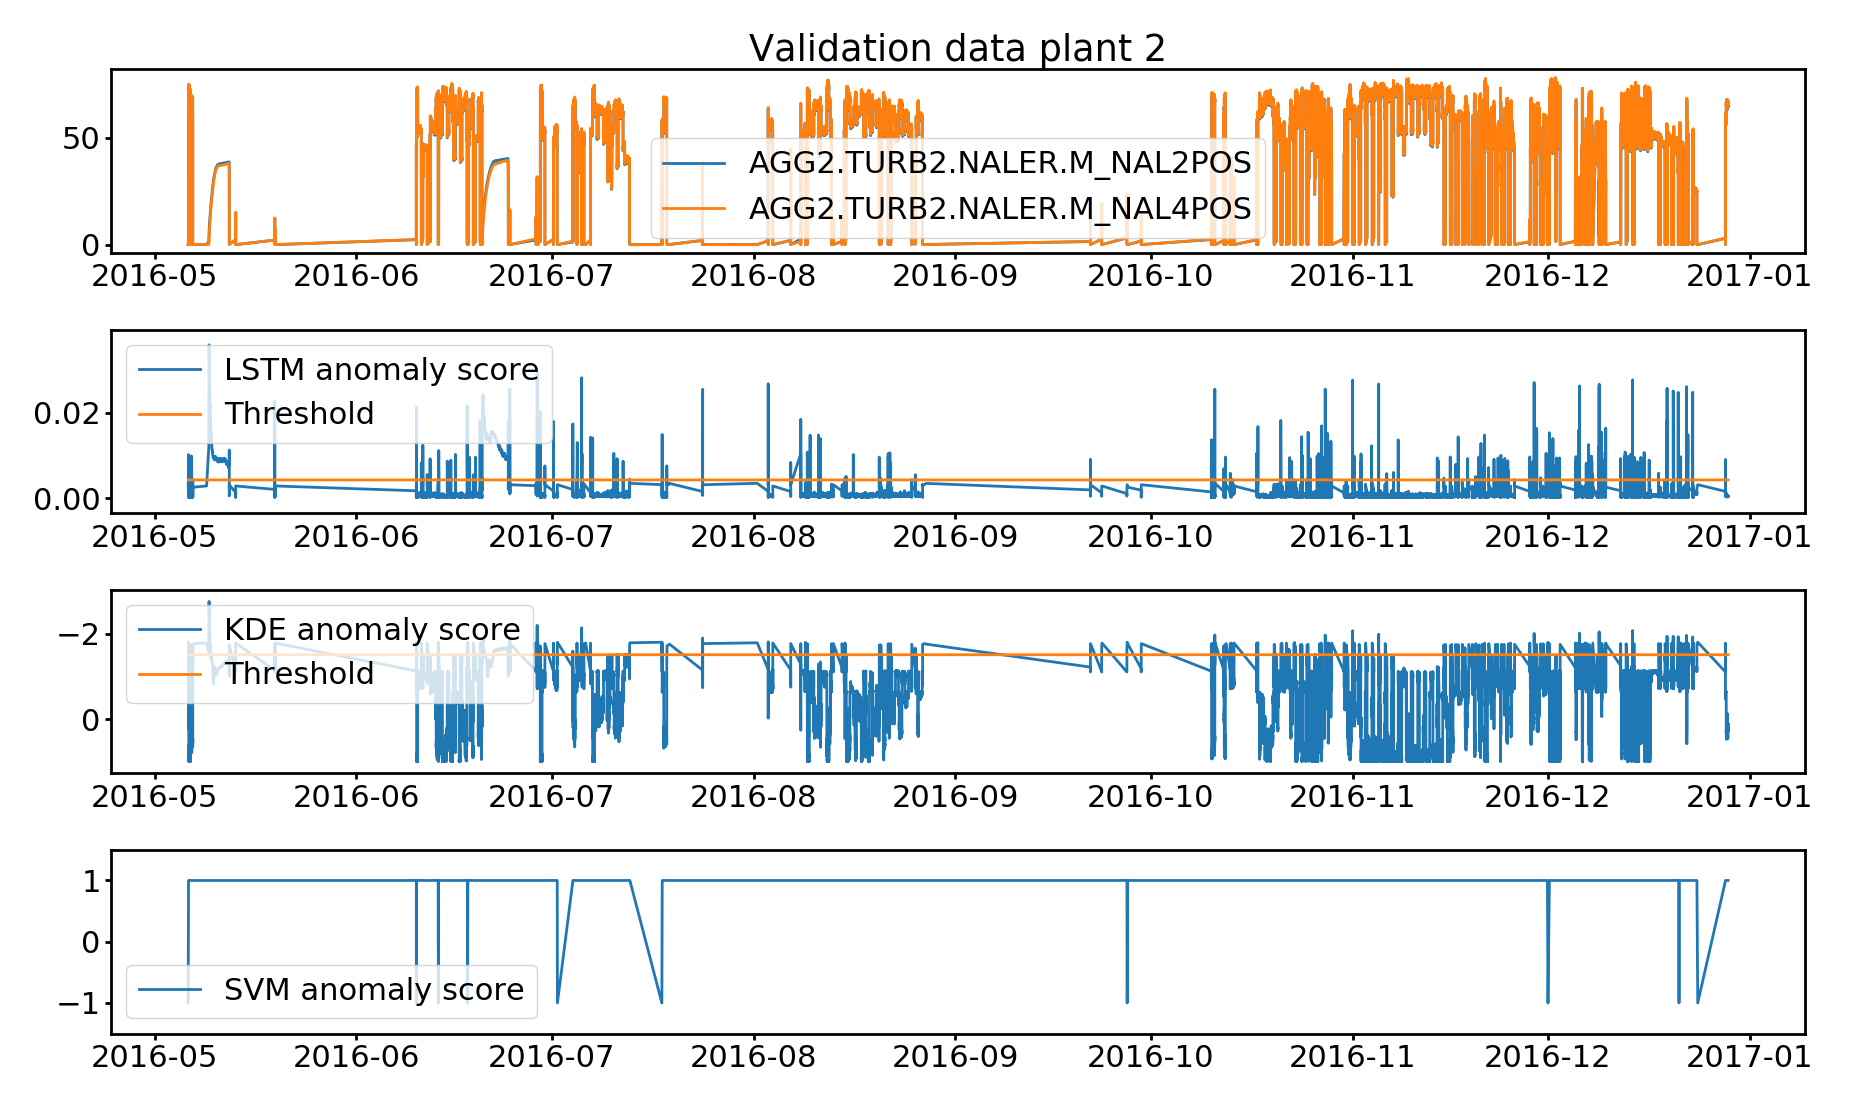
\includegraphics[width=\textwidth]{report/figures/analysis/plant2_train_long/test_data_anomaly.png}
    %         \caption{Anomaly score for the plant 2 test set, detectors trained on plant 2 long training set}
    %         \label{fig:plant2_long_test_anomaly_score}
    %     \end{figure}
        
    %     \begin{figure}
    %         \centering
    %         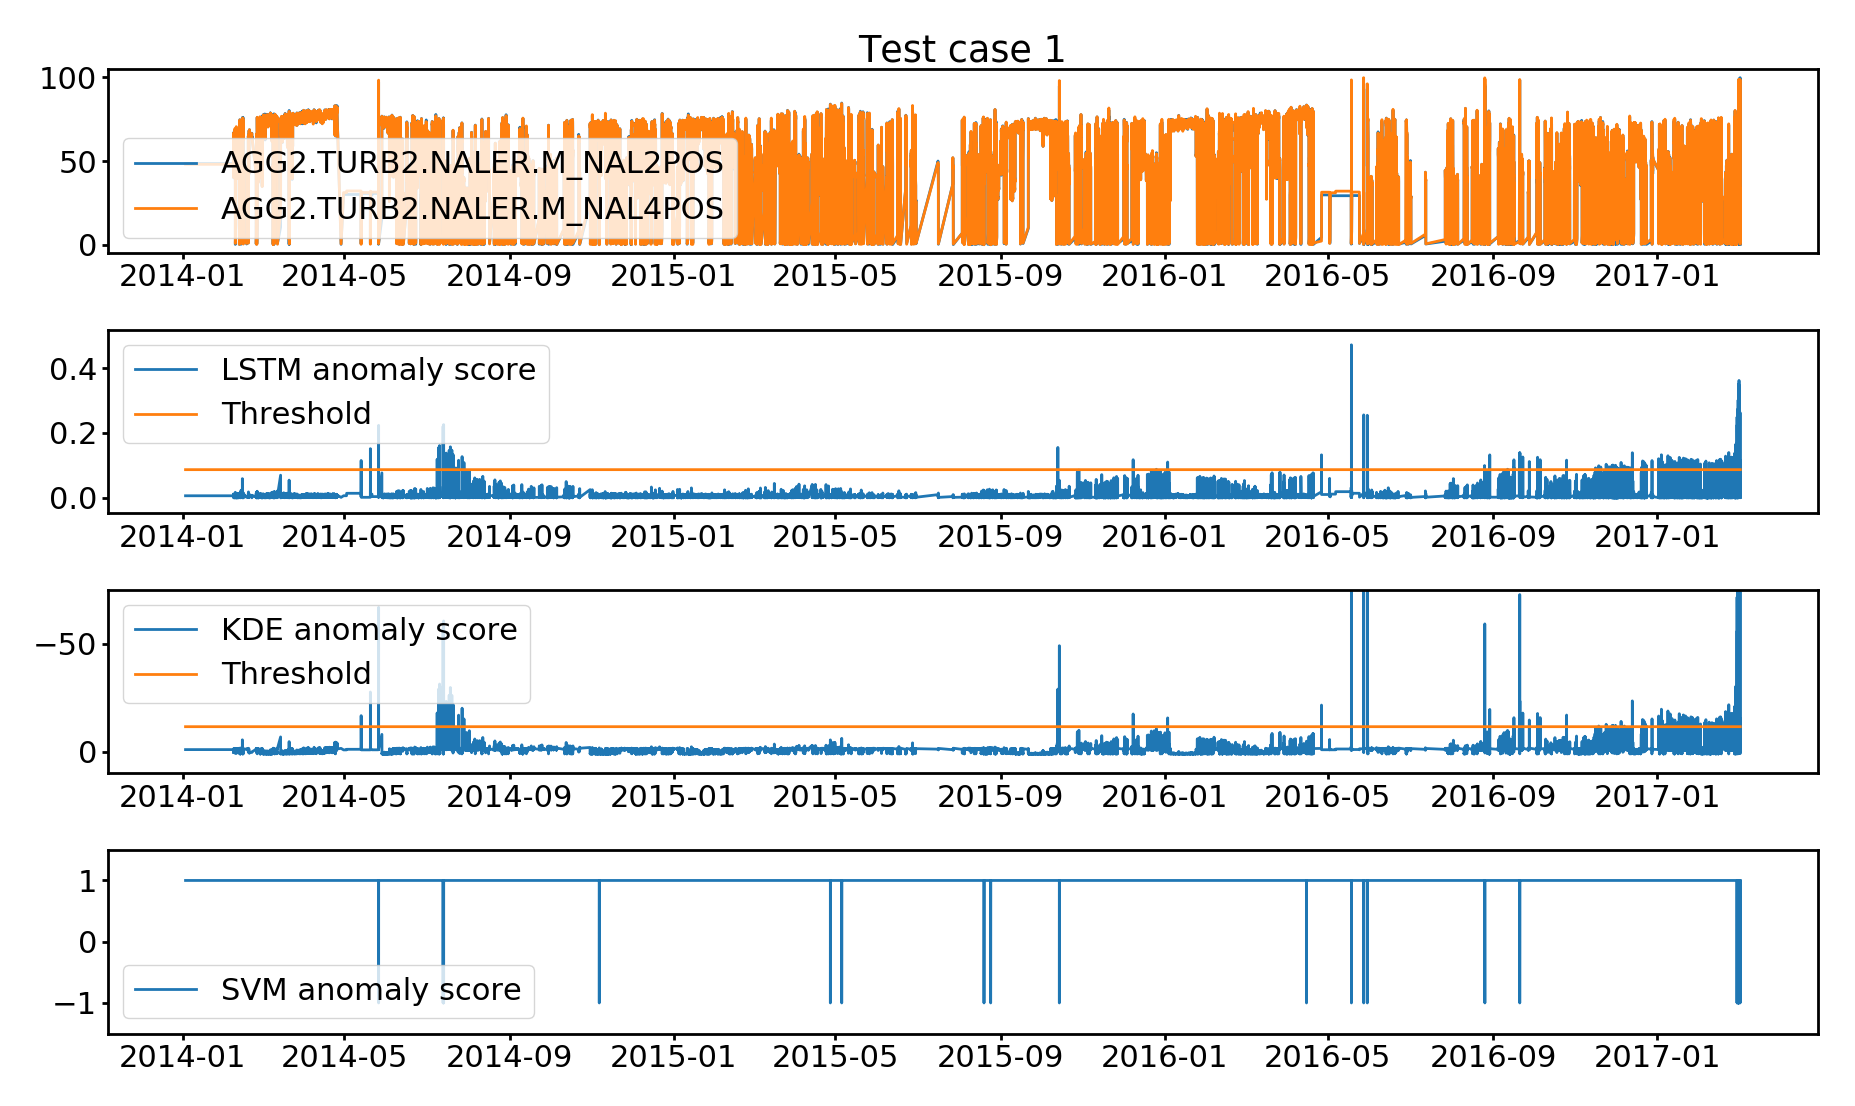
\includegraphics[width=\textwidth]{report/figures/analysis/plant2_train_long/production_data_anomaly.png}
    %         \caption{Anomaly score for the plant 1 production set, detectors trained on plant 2 long training set}
    %         \label{fig:plant2_long_production_anomaly_score}
    %     \end{figure}
    
    
    
    %     % \begin{table}[]
    %     %     \centering
    %     %     \begin{tabular}{|c|c|c|}
    %     %         \hline
    %     %         Test        & KDE       & LSTM  \\ \hline
    %     %         min         & -2.755    & 4.024e-05 \\ \hline
    %     %         max         & 0.999    & 0.0024   \\ \hline
    %     %         mean        & -0.366   & 0.000223  \\ \hline
    %     %     \end{tabular}
    %     %     \caption{Table of statistics for the test data for plant 2 long detector}
    %     %     \label{tab:production_stats_plant1train}
    %     % \end{table}
        
    %     % \begin{table}[]
    %     %     \centering
    %     %     \begin{tabular}{|c|c|c|}
    %     %         \hline
    %     %         Production          & KDE       & LSTM  \\ \hline
    %     %         min                 & -277.804   & 2.013e-05 \\ \hline
    %     %         max                 & 0.9987    & 0.0.0457   \\ \hline
    %     %         mean                & -1.1697    & 0.0.000807  \\ \hline
    %     %     \end{tabular}
    %     %     \caption{Table of statistics for the production data for plant 2 long detector}
    %     %     \label{tab:production_stats_plant1train}
    %     % \end{table}

    %     \begin{figure}
    %         \centering
    %         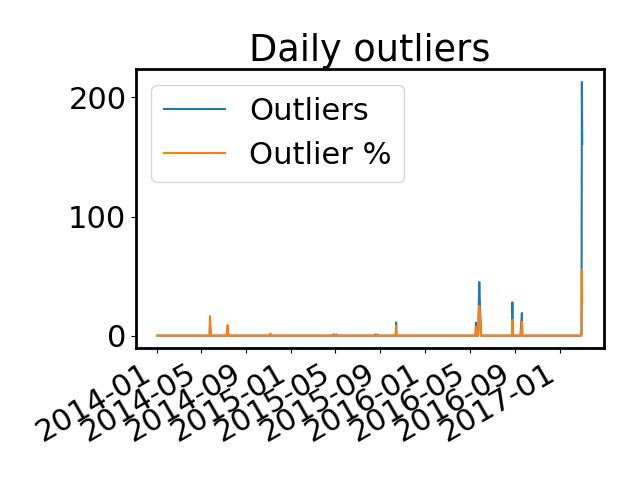
\includegraphics[width = 0.5\textwidth]{report/figures/analysis/plant2_train_long/svm_daily_outliers.png}
    %         \caption{Outlier statistics for svm}
    %         \label{fig:svm_outliers_stats}
    %     \end{figure}
        
        
    
    % \clearpage
    % \subsection{Anomaly detection 3, artificial error}
    %     The anomaly detectors trained on plant 2 are tested on the artificial error created on data from plant 2 not used for training. 
    %     \begin{figure}
    %         \centering
    %         \includegraphics[width=\textwidth]{report/figures/analysis/plant2_train_4months/plant2_artificial_anomaly_datetime.png}
    %         \caption{Anomaly score for the detectors trained on the normal data from plant 2, tested on artificial error data. The red line marks the $1\%$ most extreme scores.}
    %         \label{fig:plant2_arti_anomaly_score}
    %     \end{figure}
        
    %     As seen in figure \ref{fig:plant2_arti_anomaly_score} the detectors clearly detect the artificial error. The error is as explained above constructed to gradually increase its effect, and all three detectors are able to detect this pattern. It also looks similar to the pattern seen for the production data from plant 1. This further strengthens the claim that the error reported in March 2017, could be traced in the needle operation from early fall 2016. The artificial error is added to production data for plant $2$ from $2015$, this means that it is not seen by the detectors since they are trained from production data from $2016$.  
        
        
        
        
    % not possible to use any time-series forecasting since the data is not sampled at even frequencies. hence using a regression model and estimating an anomaly based on differences from the sampled and predicted data becomes invalid. 
    
    % bruke kde men det vil antagelig ikkje gje gode resultat sidan samplinga mi er dårlig, og eg ikkje har nok data spredd godt nok utover tilstandsrommet. 

% \section{Unsupervised dimensionallity reduction}\label{sec:dim_reduc}

%     \subsection{PCA}\label{subsec:PCA}


%     \subsection{Kernel PCA}\label{subsec:K_PCA}
    


% \section{Pelton needles}\label{sub:pelton_needles}
%     As mentioned, there was data available from three different power plants with Pelton turbines. One of the plants had recorded several issues with the needle control and was used as a case to test early detection of problems with the needle operation. 
    
    
%     \begin{figure}
%         \centering
%         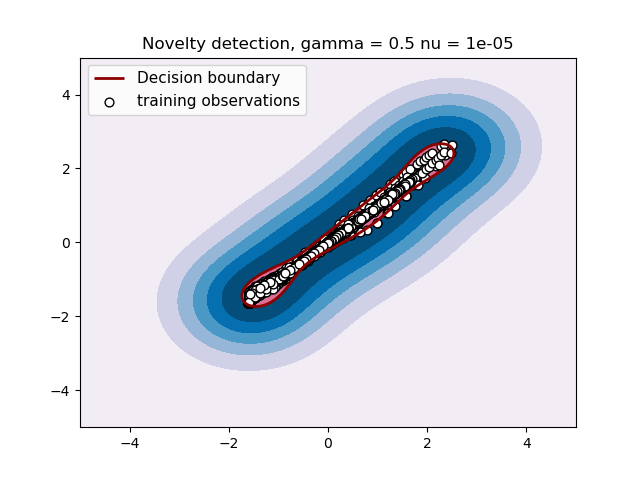
\includegraphics[scale=0.8]{report/figures/analysis/hjartdola/hjar_n2_4_novelty_05_1e-5_train.png}
%         \caption{OCSVM trained on data after overhaul in Mars 2017}
%         \label{fig:my_label}
%     \end{figure}


    
%     \begin{figure}
%         \centering
%         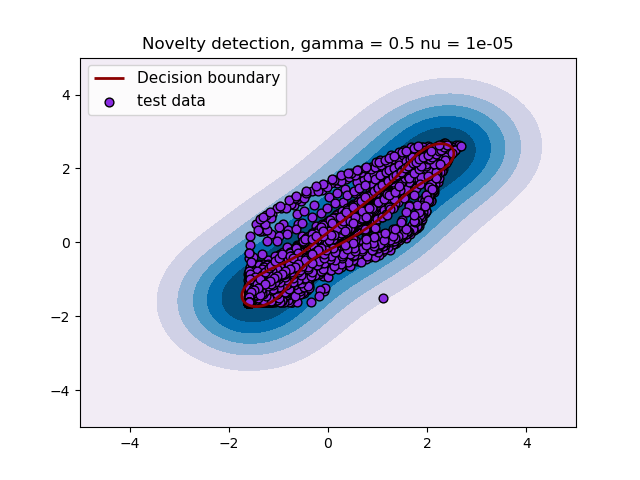
\includegraphics[scale=0.8]{report/figures/analysis/hjartdola/hjar_n2_4_novelty_05_1e-5_test.png}
%         \caption{All process data from before the overhaul}
%         \label{fig:my_label}
%     \end{figure}




% %!TEX root = ../Thesis.tex
\chapter{Discussion}\label{cha:discussion}
% %!TEX root = ../Thesis.tex
\chapter{Conclusions and future work}\label{cha:conclusions}
%
This is a summary of the results of the report, and here you also describe future work (either what you are going to do in your MSc project work, or what you would do if you had 6 more months to work on this topic.)












\section{Conclusion}


\section{Further work}

% \appendix

% \backmatter
% \addcontentsline{toc}{chapter}{\bibname}
% \bibliography{bib/bibliography}

\end{document}
